%Tex root = BasiDiDati.tex

\chapter{Esecuzione concorrente di transazioni}
L'unità di misura usata per valutare il carico di lavoro din un DBMS è il \textcolor{azzurrino}{\textbf{numero di transazioni al secondo}} (tps).\\[0.2ex]
Per gestire con prestazioni accettabili il carico di lavoro tipico delle applicazioni gestionali è di 100 o 1000 tps.\\[0.2ex]
L'esecuzione concorrente di transazioni senza controllo può generare \textbf{anomalie} o \textbf{problemi di correttezza}.\\[0.2ex]
Bisogna, quindi, introdurre dei meccanismi di controllo nell'esecuzione delle transazioni per evitare tali anomalie.

\section{Tipologie di anomalie}
Le principali tipologie di anomalie sono:
\begin{itemize}[label=$\triangleright$, itemsep=\smallskipamount]
    \item \textbf{perdita di aggiornamento}: effetti di una transazione concorrente vengono persi (riscritti)
    \item \textbf{lettura inconsistente}: accessi sucessivi alla stessa risorsa ritornano risultati diversi
    \item \textbf{lettura sporca}: viene letto un dato che rappresenta uno stato intermedio di un'altra transazione
    \item \textbf{aggiornamento fantasma}: osservazione di uno stato intermedio che viola i vincoli d'integrità
    \item \textbf{inserimento fantasma}: valutazioni diverse di operazioni di aggregazione producono risultati diversi
\end{itemize}

\vario{Notazione}{
    \begin{itemize}[label=$\diamond$, itemsep=\smallskipamount]
        \item $\mathbf{t_i}$: transazione $\mathrm{t_i}$
        \item $\mathbf{r_i(x)}$: operazione di lettura eseguita dalla transazione $\mathrm{t_i}$ sulla risorsa $\mathrm{x}$
        \item $\mathbf{w_i(x)}$: operazione di scrittura eseguita dalla transazione $\mathrm{t_i}$ sulla risorsa $\mathrm{x}$
    \end{itemize}
}

\subsection{Perdita di aggiornamento}
Nella \textbf{perdita di aggiornamento} gli effetti di una transazione concorrente vengono persi.

\esempio{perdita di aggiornamento}{
    Consieriamo le seguenti transazioni:
    \[
        \begin{aligned}
            \mathrm{t_1}:\; & \texttt{BOT}; \; \mathrm{r_1(x)}; \;\mathrm{ x = x + 1}; \; \mathrm{w_1(x)}; \; \texttt{COMMIT}; \; \texttt{EOT} \\
            \mathrm{t_2}:\; & \texttt{BOT}; \; \mathrm{r_2(x)}; \; \mathrm{x = x + 1}; \; \mathrm{w_2(x)}; \; \texttt{COMMIT}; \; \texttt{EOT}
        \end{aligned}
    \]

    Simuliamo l'esecuzione concorrente di $\mathrm{t_1}$ e $\mathrm{t_2}$:
    \begin{figure}[H]
        \centering
        \includegraphics[width=0.9\textwidth]{images/perdita-aggiornamento.png}
    \end{figure}
}

\subsection{Lettura inconsistente}
Nella \textbf{lettura inconsistente} gli accessi successivi a uno stesso dato all'interno di una transazione ritornano valori diversi.

\esempio{lettura inconsistente}{
    Consieriamo le seguenti transazioni:
    \[
        \begin{aligned}
            \mathrm{t_1}:\; & \texttt{BOT}; \; \mathrm{r_1(x)}; \; \mathrm{r_1'(x)}; \; \texttt{COMMIT}; \; \texttt{EOT} \\
            \mathrm{t_2}:\; & \texttt{BOT}; \; \mathrm{r_2(x)}; \; \mathrm{x = x + 1}; \; \mathrm{w_2(x)}; \; \texttt{COMMIT}; \; \texttt{EOT}
        \end{aligned}
    \]

    Simuliamo l'esecuzione concorrente di $\mathrm{t_1}$ e $\mathrm{t_2}$:
    \begin{figure}[H]
        \centering
        \includegraphics[width=0.9\textwidth]{images/lettura-inconsistente.png}
    \end{figure}
}

\subsection{Lettura sporca}
Nella \textbf{lettura sporca} viene letto un dato che rappresenta uno stato intermedio nell'evoluzione di una transazione.

\esempio{lettura inconsistente}{
    Consieriamo le seguenti transazioni:
    \[
        \begin{aligned}
            \mathrm{t_1}:\; & \texttt{BOT}; \; \mathrm{r_1(x)}; \; \texttt{COMMIT}; \; \texttt{EOT} \\
            \mathrm{t_2}:\; & \texttt{BOT}; \; \mathrm{r_2(x)}; \; \mathrm{x = x + 1}; \; \mathrm{w_2(x)}; \; \dots \texttt{ABORT};
        \end{aligned}
    \]

    Simuliamo l'esecuzione concorrente di $\mathrm{t_1}$ e $\mathrm{t_2}$:
    \begin{figure}[H]
        \centering
        \includegraphics[width=0.9\textwidth]{images/lettura-sporca.png}
    \end{figure}
}

\subsection{Aggiornamento fantasma}
L'\textbf{aggiornamento fantasma} consiste nell'osservazione di uno stato intermedio che non soddisfa i vincoli d'integrità.

\esempio{lettura inconsistente}{
    Consieriamo le seguenti transazioni:
    \[
        \begin{aligned}
        \text{Risorse} &: \mathrm{x, y, z} \\
        \text{Vincoli} &: \mathrm{x + y + z = 100} \\
        \end{aligned}
    \] 
    \[
        \begin{aligned}
        \mathrm{t_1}:\; & \texttt{BOT}; \; \mathrm{r_1(y)}; \; \mathrm{r_1(x)}; \; \mathrm{r_1(z)}; \; \mathrm{s = x + y + z}; \; \texttt{EOT} \\
        \mathrm{t_2}:\; & \texttt{BOT}; \; \mathrm{r_2(y)}; \; \mathrm{y = y + 10}; \; \mathrm{r_2(z)}; \; \mathrm{z = z - 10}; \; \mathrm{w_2(y)}; \; \mathrm{w_2(z)};
        \; \texttt{COMMIT}; \; \texttt{EOT}
        \end{aligned}
    \] 

    Simuliamo l'esecuzione concorrente di $\mathrm{t_1}$ e $\mathrm{t_2}$:
    \begin{figure}[H]
        \centering
        \includegraphics[width=0.9\textwidth]{images/aggiornamento-fantasma.png}
    \end{figure}
}

\subsection{Inserimento fantasma}
L'\textbf{inserimento fantasma} si verifica quando avvengono valutazioni diverse di valori aggregati a causa di inserimenti intermedi.\\[0.2ex]
La transazione che valuta un valore aggregato relativo a tutti gli elementi che soddifano un predicato di selezione (es. voto medio degli studenti) può subire l'anomalia di inserimento se il valore aggregato viene valutato due volte e tra la prima e la seconda valutazione viene inserito un nuovo studente.

\section{Schedule}
\definizione{schedule}{
    Lo \textbf{schedule} è una sequenza di operazioni di lettura e scrittura eseguite su risorse della base di dati da diverse transazioni concorrenti.
}

Lo schedule, quindi, rappresenta una possibile esecuzione concorrente di diverse transazioni:
\begin{equation*}
    \mathbf{S: r_1(x) \quad r_2(x) \quad w_1(z) \quad w_2(x)}
\end{equation*}

Per evitare anomalie, si stabilisce di accettare solo gli schedule equivalenti a uno schedule seriale.

\subsection{Schedule seriale}
\definizione{schedule seriale}{
    Uno \textbf{schedule seriale} è uno schedule dove le operazioni di ogni transazione compaiono un seuqenza senza essere inframezzate da operazioni di altre transazioni.

    \noindent\rule{\textwidth}{0.4pt}

    \medskip
    \[
        \begin{aligned}
            \mathrm{s_1}: \mathrm{r_1(x)} \quad \mathrm{r_2(x)} \quad \mathrm{w_2(x)} \quad \mathrm{w_1(x)} &= \textbf{\text{NON è SERIALE}}\\
            \mathrm{s_2}: \mathrm{r_1(x)} \quad \mathrm{w_1(x)} \quad \mathrm{r_2(x)} \quad \mathrm{w_2(x)} &= \textbf{\text{è SERIALE}}
        \end{aligned}
    \]
}

\definizione{schedule serializzabile}{
    Lo \textbf{schedule serializzabile} è uno schedule equivalente a uno schedule seriale.
}

Due schedule si definiscono equivalenti se \textbf{producono gli stessi effetti} sulla base di dati.

\section{Tecniche di gestione della concorrenza}
Per le seguenti tecniche di gestione della concorrenza, si assume l'ipotesi di \textbf{commit-proiezione} (transazioni hanno esito noto).\\[0.2ex]
Di conseguenza, vengono tolti dagli schedule tutte le operazioni delle transazioni che non vanno a buon fine.

\subsection{View-equivalenza}
\definizione{relazione \texttt{LEGGE\_DA}}{
    Dato uno schedule $\mathrm{S}$, si dice che un'operazione di lettura $\mathrm{r_i(x)}$ (che compare in $\mathrm{S}$) \texttt{LEGGE\_DA} un'operazione di scrittura $\mathrm{w_i(x)}$ (che compare in $\mathrm{S}$), se $\mathrm{w_j(x)}$ \textbf{precede} $\mathrm{r_i(x)}$ in S e non è alcuna operazione $\mathrm{w_k(x)}$ tra le due.

    \[
        \begin{aligned}
            \mathrm{S_1}: \mathrm{r_1(x)} \ \mathrm{r_2(x)} \ \mathrm{w_2(x)} \ \mathrm{w_1(x)} \quad &\texttt{LEGGE\_DA(S1)} = \emptyset\\
            \mathrm{S_2}: \mathrm{r_1(x)} \ \mathrm{w_1(x)} \ \mathrm{r_2(x)} \ \mathrm{w_2(x)} \quad &\texttt{LEGGE\_DA(S2)} = \{(\mathrm{r_2(x), w_1(x)})\}\\
            \mathrm{S_3}: \mathrm{r_1(x)} \ \mathrm{w_1(x)} \ \mathrm{w_2(x)} \ \mathrm{r_2(x)} \quad &\texttt{LEGGE\_DA(S3)} = \emptyset
        \end{aligned}
    \]
}

\definizione{scritture finali}{
    Dato uno schedule $\mathrm{S}$ si dice che un'operazione di scrittura $\mathrm{w_i(x)}$ (che compare in $\mathrm{S}$) è una \texttt{scrittura finale} se è l'ultima operazione di scrittura della risorsa $\mathrm{x}$ in $\mathrm{S}$.

    \[
       \begin{aligned}
            \mathrm{S_1}: \mathrm{r_1(x)} \ \mathrm{r_2(x)} \ \mathrm{w_2(x)} \ \mathrm{w_3(y)} \ \mathrm{w_1(x)} \quad &\texttt{SCRITTURE\_FINALI(S1)} = \{\mathrm{w_3(y)}, \mathrm{w_1(x)}\}\\
            \mathrm{S_2}: \mathrm{r_1(x)} \ \mathrm{w_1(x)} \ \mathrm{r_2(x)} \ \mathrm{w_2(x)} \ \mathrm{w_3(y)} \quad &\texttt{SCRITTURE\_FINALI(S1)} = \{\mathrm{w_2(x), w_3(y)}\}
        \end{aligned}     
    \]
}

\definizione{view-equivalenza}{
    Due schedule $\mathrm{S_1}$ e $\mathrm{S_2}$ sono \textbf{view-equivalenti} $(\mathbf{S_1} \ \mathbf{\approx_V} \ \mathbf{S_2})$ se possiedono le stesse relazioni \texttt{LEGGE\_DA} e \texttt{SCRITTURE\_FINALI}.
}

\definizione{viwe-serializzabilità}{
    Uno schedule S è \textbf{view-serializzabili} (VSR) se esiste uno schedule seriale $\mathrm{S'}$ tale che $\mathbf{S \ \approx_V \ S'}$.

    \vario{Attenzione}{
        Gli schedule seriali $\mathrm{S'}$ si generano considerando tutte le possibili permutazioni delle transazioni (non delle operazioni delle transazioni) che compaiono in $\mathrm{S}$.

        Inoltre, non si deve cambiare l'ordine delle operazioni di ciascuna transazione perchè ciò significherebbe modificare la transazione.
    }
}

Gli schedule corrispondenti alle anomalie di:
\begin{itemize}[label=$\diamond$, itemsep=\smallskipamount]
    \item perdita di aggiornamento
    \item letture inconsistenti
    \item aggiornamenti fantasmi
\end{itemize}

non sono view-serializzabili.\\[0.2ex]
Inoltre, l'algoritmo per il test di view-equivalenza tra due schedule è di complessità lineare, mentre per il test di view-serializzabilità di uno schedule è di complessità esponenziale.\\[0.2ex]
In conclusione si è osservato che la view-serializzabilità richiede l'ipotesi di commit-proiezione e algoritmi di complessità troppo elevata, quindi, non è applicabile nei sistemi reali.

\esercizio{perdita di aggiornamento}{
    Consideriamo le seguenti transazioni:
  \[
  \begin{aligned}
    \mathrm{t_1}:\; & \mathrm{r_1(x)}; \; \mathrm{w_1(x)} \\
    \mathrm{t_2}:\; & \mathrm{r_2(x)}; \; \mathrm{w_2(x)}
  \end{aligned}
  \] 
  Eseguire lo schedule:
  \[
    \mathbf{S_{pa} = r_1(x); \; r_2(x); \; w_2(x); \; w_1(x);}
  \]

  \textcolor{red}{\textbf{Questo schedule è view serializzabile?}}

  \smallskip
  Calcoliamo le relazioni:
  \begin{itemize}[label=$\triangleright$, itemsep=\smallskipamount]
    \item \texttt{LEGGE\_DA}\( (\mathrm{S_{pa}}) = \varnothing \)
    \item \texttt{SCRITTURE\_FINALI}\( (\mathrm{S_{pa}}) = \{ \mathrm{w_1(x)} \} \)
  \end{itemize}

  \smallskip
  Bisogna generare tutti i possibili schedule seriali per determinare se
  esiste uno schedule seriale \( \mathrm{S'} \) tale che \( \mathrm{S_{pa} \approx_V S'} \).

  Gli schedule seriali sono:
  \begin{itemize}[label=$\circ$, itemsep=\medskipamount]
    \item \( \mathbf{S_{12} = r_1(x); \; w_1(x); \; r_2(x); \; w_2(x);} \) 
      \begin{itemize}[itemsep=\smallskipamount]
        \item \texttt{LEGGE\_DA}\( \mathrm{(S_{12})} = \{ \mathrm{(r_2(x), w_1(x))} \} \)
        \item \texttt{SCRITTURE\_FINALI}\( \mathnormal{(S_{12})} = \{ \mathrm{w_1(x)} \} \)
      \end{itemize}
      Osserviamo che \( \mathbf{S_{pa} \not\approx_V S_{12}} \)

    \item \( \mathbf{S_{21} = r_2(x); \; w_2(x); \; r_1(x); \; w_1(x);} \) 
      \begin{itemize}[itemsep=\smallskipamount]
        \item \texttt{LEGGE\_DA}\( \mathrm{(S_{21})} = \{ \mathrm{(r_1(x), w_2(x))} \} \)
        \item \texttt{SCRITTURE\_FINALI}\( \mathrm{(S_{21})} = \{ \mathrm{w_1(x)} \} \)
      \end{itemize}
      Osserviamo che \( \mathbf{S_{pa} \not\approx_V S_{21}} \)
  \end{itemize}

  \smallskip
  Avendo provato per tutte le possibili permutazioni si può dire che lo schedule
  \( \mathrm{S_{pa}} \) \textbf{non è view-serializzabile}.
}

\esercizio{lettura inconsistente}{
    Consideriamo le seguenti transazioni:
  \[
  \begin{aligned}
    \mathrm{t_1}:\; & \mathrm{r_1(x)}; \; \mathrm{w_1(x)}; \; \mathrm{r_1(y)}; \; \mathrm{w_1(y)} \\
    \mathrm{t_2}:\; & \mathrm{r_2(z)}; \; \mathrm{r_2(x)}; \; \mathrm{w_2(x)}; \; \mathrm{w_2(z)}
  \end{aligned}
  \]

  Eseguire lo schedule:
  \[
    \mathbf{S_1 = r_1(x); \; w_1(x); \; r_2(z); \; r_1(y); \; w_1(y); \; r_2(x); \; w_2(x); \;
    w_2(z);}
  \]

  \textcolor{red}{\textbf{Questo schedule è view serializzabile?}}

  \smallskip
  Calcoliamo le relazioni:
  \begin{itemize}[label=$\triangleright$, itemsep=\smallskipamount]
    \item \texttt{LEGGE\_DA}\( \mathrm{(S_1)} = \left\{ \mathrm{(r_2(x), w_1(x))} \right\} \)
    \item \texttt{SCRITTURE\_FINALI}\( \mathrm{(S_1)} = \left\{ \mathrm{w_2(x), w_1(y), w_2(z)} \right\} \)
  \end{itemize}

  \smallskip
  Bisogna generare tutti i possibili schedule seriali per determinare se
  esiste uno schedule seriale \( \mathrm{S'} \) tale che \( \mathrm{S_1 \approx_V S'} \).

  Gli schedule seriali sono:
  \begin{itemize}[label=$\circ$, itemsep=\medskipamount]
    \item \( \mathbf{S_{12} = t_1 t_2} \) 

    \item \( \mathbf{S_{21} = t_2 t_1} \) 
  \end{itemize}

  \smallskip
  Al posto di creare tutte le permutazioni degli schedule seriali, cerchiamo di
  osservare le relazioni \texttt{LEGGE\_DA} e \texttt{SCRITTURE\_FINALI} per capire se \( \mathrm{S_1} \) è view-equivalente ad \( \mathrm{S_{12}} \) o \( \mathrm{S_{21}} \).

  Dalla presenza di \( \mathrm{w_2(x)} \) nelle scritture finali di \( \mathrm{S_1} \) si nota che
  \( \mathrm{t_1 < t_2} \) perchè \( \mathrm{w_2(x)} \) è l'ultima scrittura di \( \mathrm{x} \) in \( \mathrm{S_1} \), 
  e questa operazione viene eseguita solo da \( \mathrm{t_2} \) e di conseguenza va eseguita
  dopo \( \mathrm{t_1} \). Da ciò sappiamo che sicuramente \( \mathrm{S_1 \not\approx_V S_{21}} \) e ci rimane da controllare soltanto se \( \mathrm{S_1 \approx_V S_{12}} \):
  \[
    \mathbf{S_{12} = r_1(x); \; w_1(x); \; r_1(y); \; w_1(y); \; r_2(z); \; r_2(x); \; w_2(x); \;
    w_2(z);}
  \] 
  \begin{itemize}[label=$\triangleright$, itemsep=\smallskipamount]
    \item \texttt{LEGGE\_DA}\( \mathrm{(S_{12})} = \left\{ \mathrm{(r_2(x), w_1(x))} \right\} \)
    \item \texttt{SCRITTURE\_FINALI}\( \mathrm{(S_{12})} = \left\{ \mathrm{w_2(x), w_1(y), w_2(z)} \right\} \)
  \end{itemize}

  \smallskip
  Osserviamo che \( \mathrm{S_1 \approx_V S_{12}} \) e quindi \( \mathrm{S_1} \) è \textbf{view-serializzabile}.
}

\esercizio{}{
    Consideriamo le seguenti transazioni:
  \[
  \begin{aligned}
    \mathrm{t_1}:\; & \mathrm{r_1(x)}; \; \mathrm{w_1(x)}; \; \mathrm{r_1(y)}; \; \mathrm{w_1(y)} \\
    \mathrm{t_2}:\; & \mathrm{r_2(z)}; \; \mathrm{r_2(x)}; \; \mathrm{w_2(x)}; \; \mathrm{w_2(z)}
  \end{aligned}
  \]

  Eseguire lo schedule:
  \[
    \mathbf{S_1 = r_1(x); \; w_1(x); \; r_2(z); \; r_1(y); \; w_1(y); \; r_2(x); \; w_2(x); \;
    w_2(z);}
  \]

  \textcolor{red}{\textbf{Questo schedule è view serializzabile?}}

  \smallskip
  Calcoliamo le relazioni:
  \begin{itemize}[label=$\triangleright$, itemsep=\smallskipamount]
    \item \texttt{LEGGE\_DA}\( \mathrm{(S_1)} = \left\{ \mathrm{(r_2(x), w_1(x))} \right\} \)
    \item \texttt{SCRITTURE\_FINALI}\( \mathrm{(S_1)} = \left\{ \mathrm{w_2(x), w_1(y), w_2(z)} \right\} \)
  \end{itemize}

  \smallskip
  Bisogna generare tutti i possibili schedule seriali per determinare se esiste uno schedule seriale \( \mathrm{S'} \) tale che \( \mathrm{S_1 \approx_V S'} \).

  Gli schedule seriali sono:
  \begin{itemize}[label=$\circ$, itemsep=\medskipamount]
    \item \( \mathbf{S_{12} = t_1 t_2} \) 

    \item \( \mathbf{S_{21} = t_2 t_1} \) 
  \end{itemize}

  \smallskip
  Al posto di creare tutte le permutazioni degli schedule seriali, cerchiamo di
  osservare le relazioni \texttt{LEGGE\_DA} e \texttt{SCRITTURE\_FINALI} per capire se \( \mathrm{S_1} \) è view-equivalente ad \( \mathrm{S_{12}} \) o \( \mathrm{S_{21}} \).

  Dalla presenza di \( \mathrm{w_2(x)} \) nelle scritture finali di \( \mathrm{S_1} \) si nota che \( \mathrm{t_1 < t_2} \) perchè \( \mathrm{w_2(x)} \) è l'ultima scrittura di \( \mathrm{x} \) in \( \mathrm{S_1} \) e questa operazione viene eseguita solo da \( \mathrm{t_2} \) e di conseguenza va eseguita dopo \( \mathrm{t_1} \).
  
  Da ciò sappiamo che sicuramente \( \mathrm{S_1 \not\approx_V S_{21}} \) e ci rimane da controllare soltanto se \( \mathrm{S_1 \approx_V S_{12}} \):
  \[
    \mathbf{S_{12} = r_1(x); \; w_1(x); \; r_1(y); \; w_1(y); \; r_2(z); \; r_2(x); \; w_2(x); \;
    w_2(z)};
  \]
  \begin{itemize}
    \item \texttt{LEGGE\_DA}\( \mathrm{(S_{12})} = \left\{ \mathrm{(r_2(x), w_1(x))} \right\} \)
    \item \texttt{SCRITTURE\_FINALI}\( \mathrm{(S_{12})} = \left\{ \mathrm{w_2(x), w_1(y), w_2(z)} \right\} \)
  \end{itemize}

  \smallskip
  Osserviamo che \( \mathrm{S_1 \approx_V S_{12}} \) e quindi \( \mathrm{S_1} \) è \textbf{view-serializzabile}.
}

\esercizio{view-serializzabilità}{
  Consideriamo le seguenti transazioni:
  \[
    \begin{aligned}
      \mathrm{t_1}:\; & \mathrm{r_1(x)}; \; \mathrm{w_1(x)}; \; \mathrm{w_1(y)} \\
      \mathrm{t_2}:\; & \mathrm{r_2(y)}; \; \mathrm{r_2(x)} \\
      \mathrm{t_3}:\; & \mathrm{w_3(x)}; \; \mathrm{r_3(y)}; \; \mathrm{w_3(y)}
    \end{aligned}
  \]

  Eseguire lo schedule:
  \[
    \mathbf{S_2 = r_1(x); \; w_1(x); \; w_3(x); \; r_2(y); \; r_3(y); \; w_3(y); \; w_1(y); \;
    r_2(x)}
  \]

  \textcolor{red}{\textbf{Questo schedule è view serializzabile?}}

  \smallskip
  Calcoliamo le relazioni:
  \begin{itemize}[label=$\triangleright$, itemsep=\smallskipamount]
    \item \texttt{LEGGE\_DA}\( \mathrm{(S_2)} = \left\{ \mathrm{(r_2(x), w_3(x))} \right\} \)
    \item \texttt{SCRITTURE\_FINALI}\( \mathrm{(S_2)} = \left\{ \mathrm{w_3(x), w_1(y)} \right\} \)
  \end{itemize}

  \smallskip
  Siccome ci sono 6 possibili permutazioni vediamo se è possibile scartarne alcune
  a priori.
  \begin{itemize}[label=$\circ$, itemsep=\medskipamount]
    \item insieme \texttt{SCRITTURE\_FINALI}\( \mathrm{(S_2)} \) implica:
      \begin{itemize}[itemsep=\smallskipamount]
        \item \( \mathrm{t_1 < t_3} \) perchè \( \mathrm{w_3(x)} \) è l'ultima scrittura di \( \mathrm{x} \) in \( \mathrm{S_2} \) e questa operazione viene eseguita solo da \( \mathrm{t_3} \) e di conseguenza va eseguita dopo \( \mathrm{t_1} \)

        \item \( \mathrm{t_3 < t_1} \) perchè \( \mathrm{w_1(y)} \) è l'ultima scrittura di \( \mathrm{s} \) in \( \mathrm{S_2} \) e questa operazione viene eseguita solo da \( \mathrm{t_1} \) e di conseguenza va eseguita dopo \( \mathrm{t_3} \)
      \end{itemize}
      Si osserva che \( \mathrm{t_1 < t_3} \) e \( \mathrm{t_3 < t_1} \) è una contraddizione, cioè non esiste uno schedule seriale che le rispetti entrambe e quindi si può concludere che \( \mathrm{S_2} \) \textbf{non è view-serializzabile}.

    \item insieme \texttt{LEGGE\_DA}\( \mathrm{(S_2)} \) implica:
      \begin{itemize}[itemsep=\smallskipamount]
        \item \( \mathrm{t_3 < t_2} \) perchè \( \mathrm{r_2(x)} \) (in \( \mathrm{t_2} \)) legge da \( \mathrm{w_3(x)} \) (in \( \mathrm{t_3} \)) e quindi \( \mathrm{(r_2(x), w_3(x))} \in \texttt{LEGGE\_DA} \) 

        \item \( \mathrm{t_1 < t_3} \) per garantire \( \mathrm{(r_1(x), w_3(x))} \notin \texttt{LEGGE\_DA} \)
        \item \( \mathrm{t_2 < t_3} \) per garantire \( \mathrm{(r_2(x), w_3(x))} \in \texttt{LEGGE\_DA} \)
        \item \( \mathrm{t_2 < t_1} \) per garantire \( \mathrm{(r_2(x), w_1(x))} \notin \texttt{LEGGE\_DA} \)
        \item \( \mathrm{t_3 < t_1} \) per garantire \( \mathrm{(r_3(x), w_1(x))} \notin \texttt{LEGGE\_DA} \)
      \end{itemize}

      \smallskip
      Si osserva che \( \mathrm{t_1 < t_3} \) e \( \mathrm{t_3 < t_1} \) è una contraddizione, quindi, si può concludere che \( \mathrm{S_2} \) \textbf{non è view-serializzabile}.
  \end{itemize}
}

\esercizio{view-serializzabilità}{
  Consideriamo le seguenti transazioni:
  \[
    \begin{aligned}
      \mathrm{t_1}:\; & \mathrm{r_1(x)}; \; \mathrm{w_1(x)}; \; \mathrm{w_1(y)}; \; \mathrm{w_1(z)} \\
      \mathrm{t_2}:\; & \mathrm{r_2(x)}; \; \mathrm{w_2(x)} \\
      \mathrm{t_3}:\; & \mathrm{r_3(x)}; \; \mathrm{w_3(y)}; \; \mathrm{w_3(x)} \\
      \mathrm{t_4}:\; & \mathrm{r_4(z)} \\
      \mathrm{t_5}:\; & \mathrm{w_5(x)}; \; \mathrm{w_5(y)}; \; \mathrm{r_5(z)}
    \end{aligned}
  \]

  Eseguire con lo schedule:
  \[
    \begin{aligned}
      S_3 =& r_1(x); \; r_2(x); \; w_2(x); \; r_3(x); \; r_4(z); \; w_1(x); \; w_3(y); \;
      w_3(x); \; w_1(y); \\
          &\; w_5(x); \; w_1(z); \; w_5(y); \; r_5(z)
    \end{aligned}
  \]

  \textcolor{red}{\textbf{Questo schedule è view serializzabile?}}

  \smallskip
  Calcoliamo le relazioni:
  \begin{itemize}[label=$\triangleright$, itemsep=\smallskipamount]
    \item \texttt{LEGGE\_DA}\( (\mathrm{S_3}) = \left\{ \mathrm{(r_3(x), w_2(x)), (r_5(z), w_1(z))} \right\} \)
    \item \texttt{SCRITTURE\_FINALI}\( (\mathrm{S_3}) = \left\{ \mathrm{w_5(x), w_5(y), w_1(z)} \right\} \)
  \end{itemize}

  \smallskip
  Le permutazioni di tutte le transazioni sono \( 5! \) e, quindi, è necessario cercare
  di scartarne alcune:
  \begin{itemize}[label=$\circ$, itemsep=\medskipamount]
    \item Considerando \texttt{SCRITTURE\_FINALI}\( (\mathrm{S_3}) \) si ha che:
      \begin{itemize}[itemsep=\smallskipamount]
        \item \( \mathrm{w_5(x)} \Rightarrow \mathrm{t_2 < t_5,\; t_1 < t_5,\; t_3 < t_5} \) 
        \item \( \mathrm{w_5(y)} \Rightarrow \mathrm{t_3 < t_5,\; t_1 < t_5}\) 
      \end{itemize}
      Da queste informazioni non si rilevano contraddizioni, quindi, si procede con
      l'analisi di \texttt{LEGGE\_DA}\( (S_3) \).

    \item Considerando \texttt{LEGGE\_DA}\( (S_3) \) si ha che:
      \begin{itemize}[itemsep=\smallskipamount]
        \item \( \mathrm{(r_3(x), w_2(x))} \Rightarrow \mathrm{t_2 < t_3} \)
        \item \( \mathrm{(r_5(z), w_1(z))} \Rightarrow \mathrm{t_1 < t_5} \)
      \end{itemize}
      Da queste informazioni non si rilevano contraddizioni, quindi, si procede
      osservando cosa \textbf{non compare} nell'insieme \texttt{LEGGE\_DA}\( (\mathrm{S_3}) \):
      \begin{itemize}[itemsep=\smallskipamount]
        \item \( \mathrm{(r_1(x), w_2(x))} \notin \texttt{LEGGE\_DA}(\mathrm{S_3}) \Rightarrow
           \mathrm{t_1 < t_2} \)

         \item \( \mathrm{(r_1(x), w_3(x))} \notin \texttt{LEGGE\_DA}(\mathrm{S_3}) \Rightarrow
           \mathrm{t_1 < t_3} \)

         \item \( \mathrm{(r_1(x), w_5(x))} \notin \texttt{LEGGE\_DA}\mathrm{(S_3)} \Rightarrow
           \mathrm{t_1 < t_5} \)

         \item \( \mathrm{(r_2(x), w_1(x))} \notin \texttt{LEGGE\_DA}\mathrm{(S_3)} \Rightarrow
           \mathrm{t_2 < t_1} \)
       \end{itemize}
  \end{itemize}

  \smallskip
  Questo è in contraddizione con \( \mathrm{t_1 < t_2} \) e si può concludere che \( \mathrm{S_3} \) \textbf{non è view-serializzabile}.
}

\subsection{Conflict-equivalenza}
\definizione{conflitto}{
    Dato uno schedule $\mathrm{S}$, si dice che una coppia di operazioni $\mathrm{(a_i, a_j)}$, dove $\mathrm{a_i}$ e $\mathrm{a_j}$ compaiono nello schedule $\mathrm{S}$, rappresentano un conflitto se:
    \begin{itemize}[label=$\circ$, itemsep=\smallskipamount]
        \item appartengono a transazioni diverse $\mathrm{(i \neq j)}$
        \item entrambe operano sulla stessa risorsa
        \item almeno una di esse è un'operazione di scrittura
        \item $\mathrm{a_i}$ comapare in $\mathrm{S}$ prima di $\mathrm{a_j}$
    \end{itemize}
}

\definizione{conflit-equivalenza}{
    Due schedule $\mathrm{S_1}$ e $\mathrm{S_2}$ sono \textbf{conflit-equivalenti} ($\mathbf{S_1 \ \approx_C \ S_2}$) se possiedono le stesse operazioni e gli stessi conflitti, cioè se le operazioni in conflitto sono nello stesso ordine nei due schedule.
}

\definizione{conflict-serializzabile}{
    Uno schedule $\mathrm{S}$ è \textbf{conflit-serializzabile} (CSR) se esiste uno schedule seriale $\mathrm{S'}$ tale che $\mathrm{S \ \approx_C \ S'}$.
}

L'algoritmo per il test di conflit-serializzabilità di uno schedule è di complessità linerare.

\smallskip
Dato il seguente schedule $\mathrm{S}$:
\begin{itemize}[label=$\diamond$, itemsep=\smallskipamount]
    \item si costruisce il grafo dei conflitti $\mathrm{G(N,A)}$ dove:
    \begin{itemize}[label=$\triangleright$, itemsep=\smallskipamount]
        \item $\mathrm{N = t_1 \dots t_n}$: insieme delle transazioni di $\mathrm{S}$
        \item $\mathrm{(t_i, t_j) \in A}$ se esiste almeno un conflitto ($\mathrm{a_i, a_j}$) in $\mathrm{S}$
    \end{itemize}
    \item \textbf{se il grafo è aciclico} $\Rightarrow \mathbf{S}$ \textbf{è conflit-serializzabile}
    
    \vario{Dimostrazione}{
        \begin{enumerate}[itemsep=\medskipamount]
            \item se $\mathrm{S}$ è CSR, cioè esiste uno schdeule $\mathrm{S_R}$ seriale tale che $\mathrm{S \ \approx_C S_r}$, allora il suo grafo è aciclico.
            
            \smallskip
            \textbf{Ipotesi}: le transazioni di $\mathrm{S_r}$ sono ordinate:
            \[
                \mathrm{t_1, t_2, \dots, t_n}
            \]

            Poichè $\mathrm{S \ \approx_C S_r}$, allora $\mathrm{S_r}$ ha tutti i conflitti di $\mathrm{S}$ con operazioni esattamente nello stesso ordine.

            Quindi nel grafo dei conflitti di $\mathrm{S_r}$, ci possono essere solo archi ($\mathrm{i,j}$) con $\mathrm{i<j}$ e, questo, vuol dire che non possono esserci cicli poichè un ciclo richiederebbe un arco ($\mathrm{i,j}$) con $\mathrm{j > i}$ che è impossibile.

            Siccome $\mathrm{S \ \approx_C S_r}$, allora hanno lo stesso grafo dei conflitti e, quindi, anche il grafo dei conflitti di $\mathrm{S}$ è aciclico.
            \item se il grafo $\mathrm{S}$ è aciclico, allora $\mathrm{S}$ è CSR cioè esiste uno schdeule $\mathrm{S_R}$ seriale tale che $\mathrm{S \ \approx_C S_r}$ e, quindi, $\mathrm{S}$ e $\mathrm{S_R}$ hanno gli stessi conflitti e, quindi, lo stesso grafo.
            
            \smallskip
            \textbf{Ipotesi}: il grafo dei conflitti di $\mathrm{S}$ è aciclico e, quindi, esiste un ordinamento topologico, cioè un'enumerazione dei nodi tale che il garfo contiene solo archi ($\mathrm{i, j}$) con $\mathrm{i < j}$.

            Utilizzando questo ordinamento toplogico possiamo definire un ordine delle transazioni che produce lo stesso grafo e, quindi, siccome le transazioni sono ordinate si ha uno schdeule seriale.
        \end{enumerate}
    }
\end{itemize}

Richede comunque l'ipotesi di commit-proiezione.

\esempio{perdita di aggiornamento}{
    Consideriamo le seguenti transazioni:
  \[
    \begin{aligned}
      \mathrm{t_1}:\; & \mathrm{r_1(x)}; \; \mathrm{w_1(x)} \\
      \mathrm{t_2}:\; & \mathrm{r_2(x)}; \; \mathrm{w_2(x)}
    \end{aligned}
  \]

  Eseguire lo schedule:
  \[
    \mathbf{S_{pa}:\; r_1(x); \; r_2(x); \; w_2(x); \; w_1(x);}
  \]

  \smallskip
  L'insieme dei conflitti è:
  \[
    CONFLITTI(\mathrm{S_{pa}}) = \left\{ (\mathrm{r_1(x), w_2(x)),\; (r_2(x), w_1(x)),\; (w_2(x), w_1(x)}) \right\}
  \]

  Generiamo il grafo dei conflitti:
  \begin{figure}[H]
    \centering
    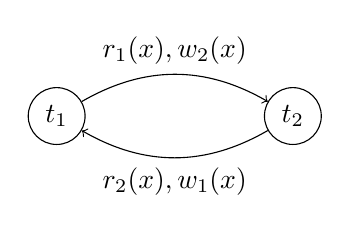
\begin{tikzpicture}
      \node[circle, draw] (t1) at (0,0) {\( t_1 \)};
      \node[circle, draw] (t2) at (3,0) {\( t_2 \)};

      \draw[->] (t1) edge [bend left] node[above] {\( r_1(x), w_2(x) \)} (t2);
      \draw[->] (t2) edge [bend left] node[below] {\( r_2(x), w_1(x) \)} (t1);
    \end{tikzpicture}
  \end{figure}

  \smallskip
  Siccome il grafo ha un ciclo \( \mathrm{S_{pa}} \) \textbf{non è conflict-serializzabile}.
}

\esempio{lettura inconsistente}{
    Consideriamo le seguenti transazioni:
  \[
    \begin{aligned}
      \mathrm{t_1}:\; & \mathrm{r_1(x)}; \; \mathrm{r'_1(x)} \\
      \mathrm{t_2}:\; & \mathrm{r_2(x)}; \; \mathrm{w_2(x)}
    \end{aligned}
  \]

  Eseguire lo schedule:
  \[
    \mathbf{S_{pa}:\; r_1(x); \; r_2(x); \; w_2(x); \; r'_1(x);}
  \]

  \smallskip
  L'insieme dei conflitti è:
  \[
    CONFLITTI(\mathrm{S_{pa}}) = \left\{ (\mathrm{r_1(x), w_2(x)),\; (w_2(x), r'_1(x)}) \right\}
  \]

  Generiamo il grafo dei conflitti:
  \begin{figure}[H]
    \centering
    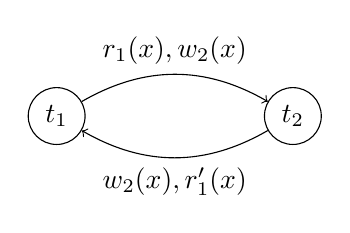
\begin{tikzpicture}
      \node[circle, draw] (t1) at (0,0) {\( t_1 \)};
      \node[circle, draw] (t2) at (3,0) {\( t_2 \)};

      \draw[->] (t1) edge [bend left] node[above] {\( r_1(x), w_2(x) \)} (t2);
      \draw[->] (t2) edge [bend left] node[below] {\( w_2(x), r'_1(x) \)} (t1);
    \end{tikzpicture}
  \end{figure}
}

\teorema{conflict-serializzabile}{
    La conflict-serializzabilità è una condizione sufficiente, ma non necessaria per la view-serializzabilità, cioè:
    \[
        \mathrm{CSR \subset VSR}
    \]

    \begin{figure}[H]
     \centering
     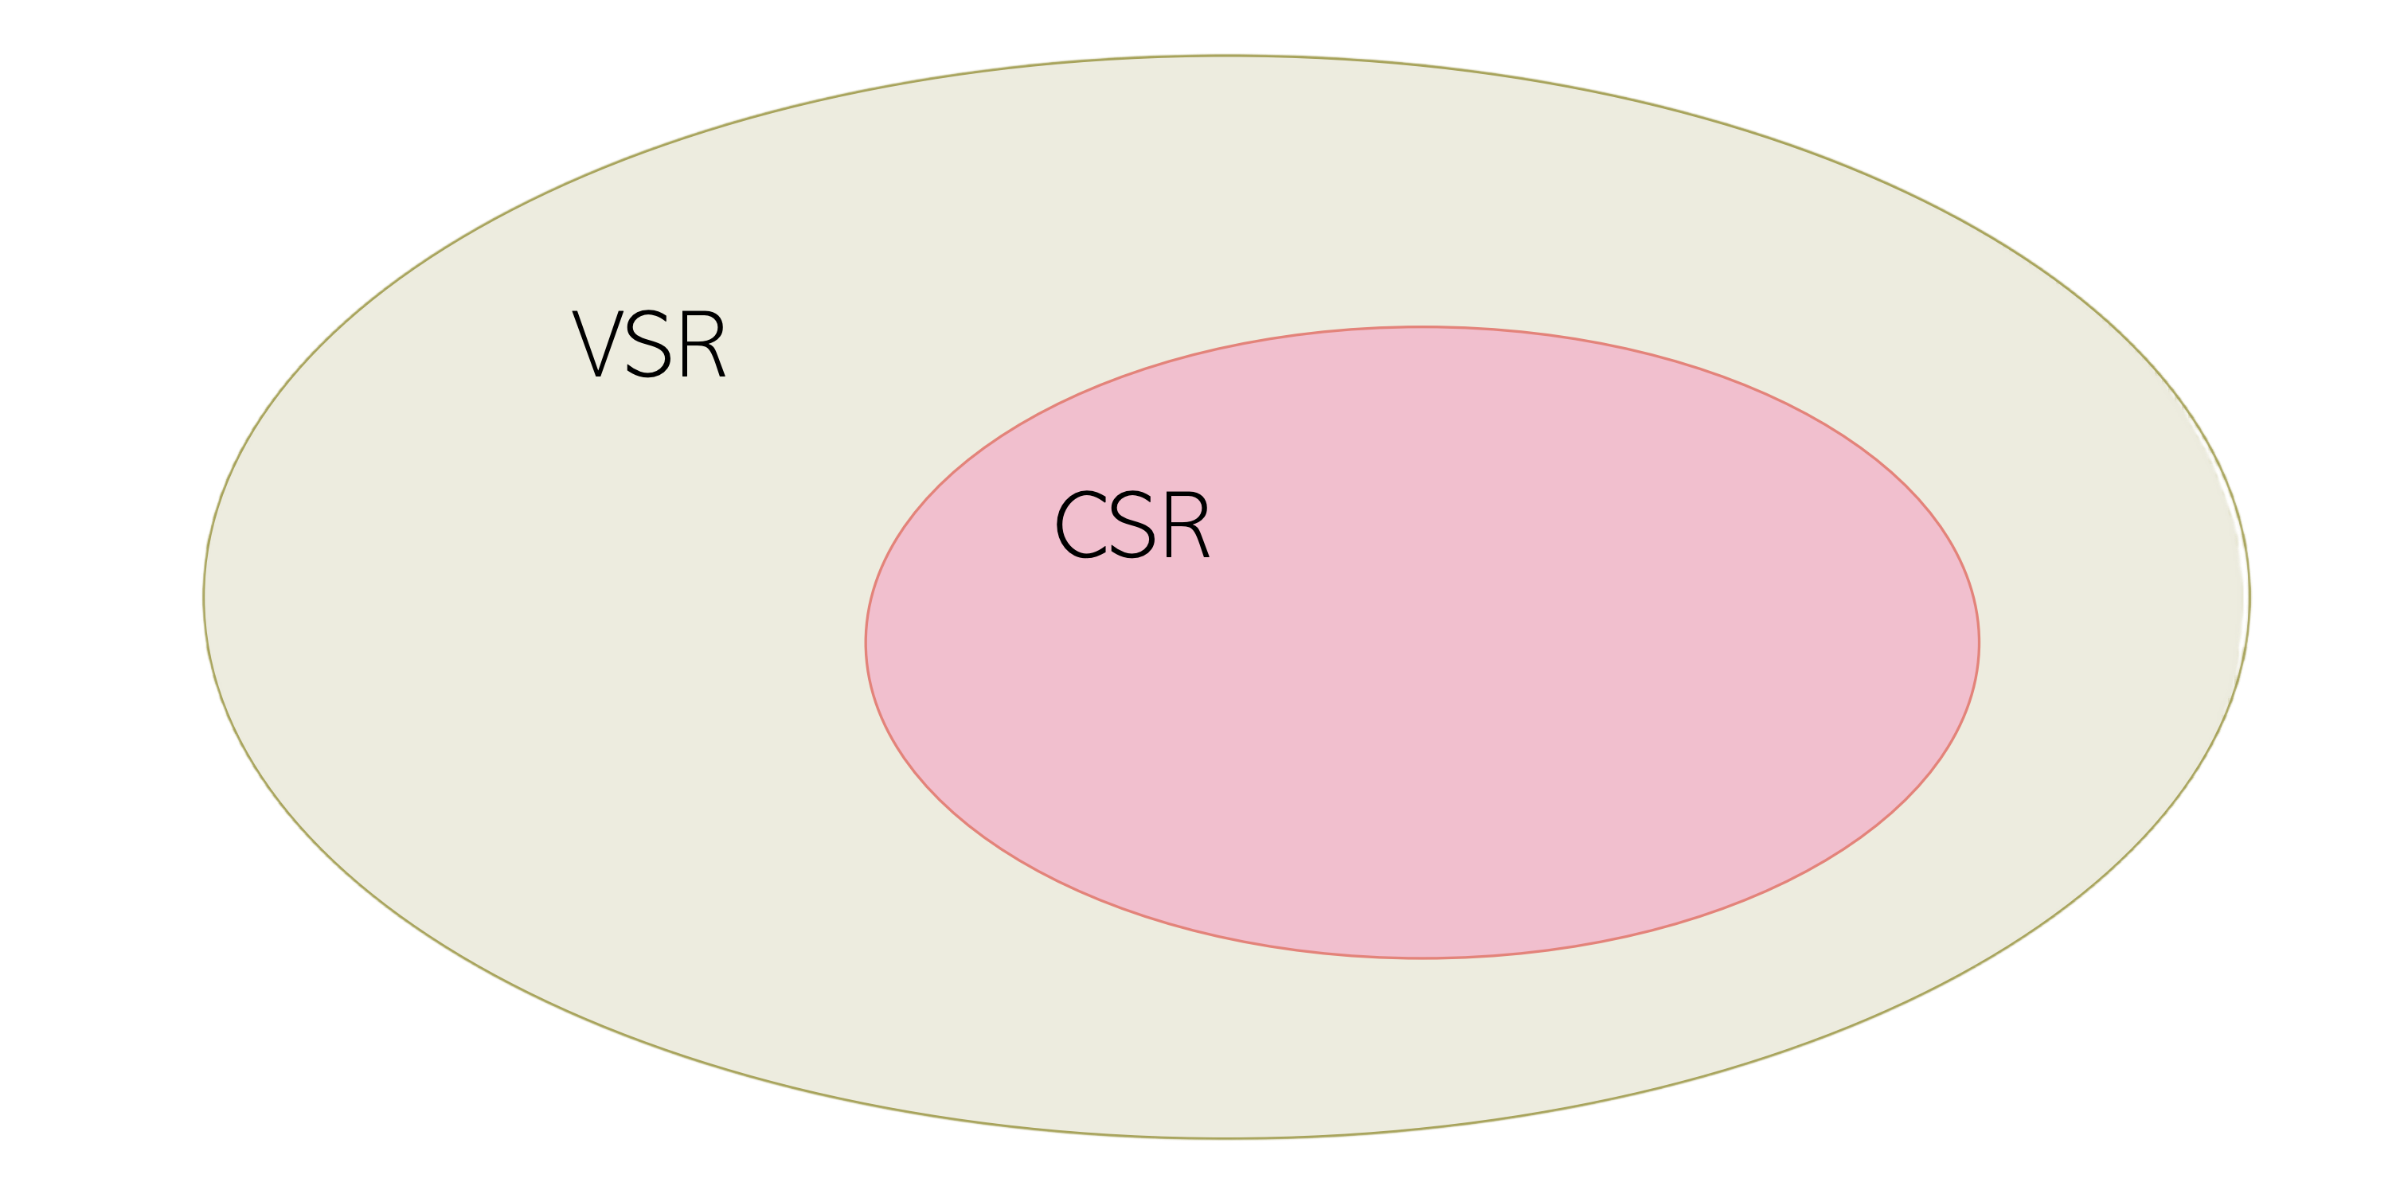
\includegraphics[width=0.5\textwidth]{images/VSR-CSR.png}
     \caption{relazione tra conflict-serializzabilità e view-serializzabilità}   
    \end{figure}

    \textbf{Dimostrazione}

    S è CSR $\Rightarrow$ S è VSR (se S non è CSR, allora non si può dire nulla sulla VSR).

    \begin{itemize}[label=$\triangleright$, itemsep=\medskipamount]
        \item \textbf{dimostrazione che} $\mathbf{CSR \subset VSR}$: basta trovare un controesempio
        \[
            \mathbf{S \in VSR} \text{ ma } \mathbf{S \notin CSR}
        \]

        Consideriamo:
        \[
           \mathrm{ S = r_1(x); w_2(x); w_1(x); w_3(x)}
        \]

        Gli insiemi sono:
        \begin{itemize}[label=$\diamond$, itemsep=\smallskipamount]
            \item \texttt{LEGGE\_DA(S)} = $\emptyset$
            \item \texttt{SCRITTURE\_FINALI(S)} = $\{\mathrm{w_3(x)}\}$
        \end{itemize}

        \smallskip
        Quindi questo schdeule è VSR perchè esiste uno schdeule $\mathrm{S_r}$ tale che $\mathrm{S_r \ \approx_V S}$:
        \[
            \mathrm{S_r = r_1(x); w_2(x); w_1(x); w_3(x)}
        \]

        che ha gli stessi insiemi:
        \begin{itemize}[label=$\diamond$, itemsep=\smallskipamount]
            \item \texttt{LEGGE\_DA($\mathrm{S_r}$)} = $\emptyset$
            \item \texttt{SCRITTURE\_FINALI($\mathrm{S_r}$)} = $\{\mathrm{w_3(x)}\}$
        \end{itemize}

        \smallskip
        Ora dimostriamo che questo schdeule non è CSR.

        Il suo insieme dei conflitti è:
        \[
            \begin{aligned}
                \texttt{CONFLITTI(S)} &= \{(\mathrm{r_1(x), w_2(x)), (r_1(x), w_3(x)), (w_2(x), w_1(x)), (w_2(x), w_3(x)})\}\\
                &= \{(\mathrm{w_1(x), w_3(x)})\}
            \end{aligned}
        \]

        Costruiamo il grafico dei conflitti:
        \begin{figure}[H]
            \centering
            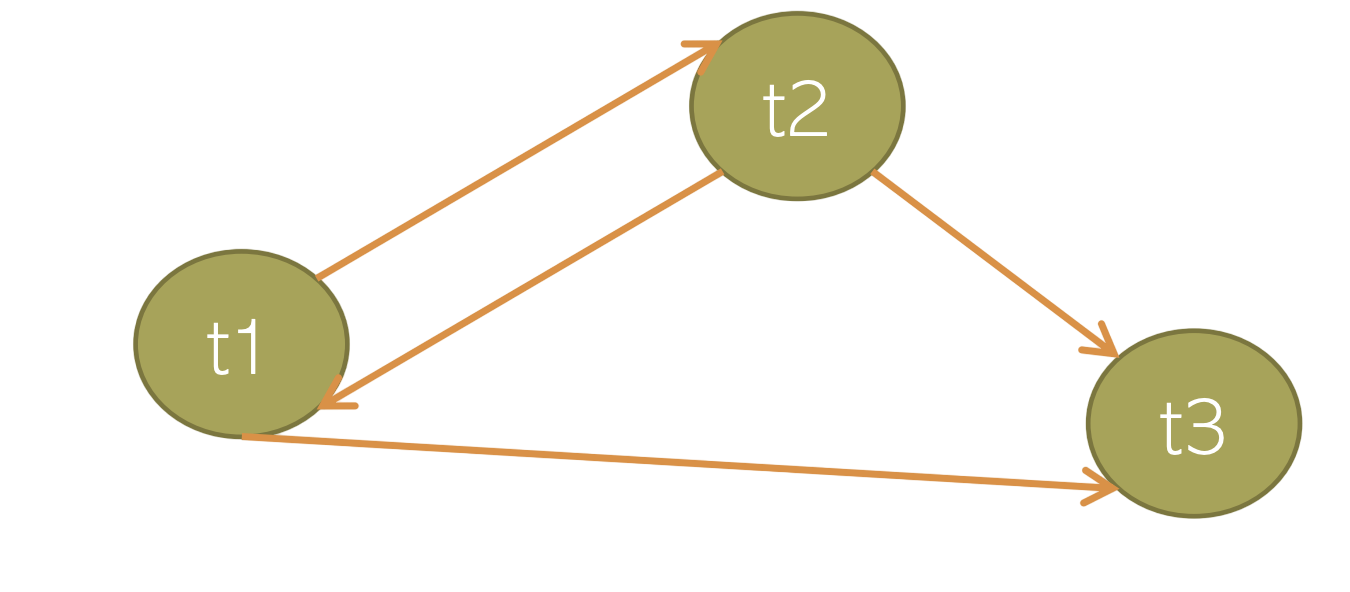
\includegraphics[width=0.45\textwidth]{images/grafico-conflitti.png}
        \end{figure}

        \item \textbf{dimostrazione che} $\mathbf{CSR \Rightarrow VSR}$: ($S_1 \approx_C S_2$ e $s_1 \approx_V S_2$)
        \begin{itemize}[label=$\circ$, itemsep=\medskipamount]
            \item $\mathrm{S_1}$ e $\mathrm{S_2}$ devono avere lo stesso insieme di \texttt{SCRITTURE\_FINALI}, altrimenti ci sarebbero due scritture sulla stessa risorsa da parte di transazioni in un ordine diverso e questo produrebbe un conflitto diverso
            \item devono avere lo stesso insieme di \texttt{LEGGE\_DA}, altrimenti ci sarebbe un conflitto, composto da una lattera e una scrittura, diverso e, quindi, siccome il conflitto è diverso, allora $\mathrm{S_1}$ e $\mathrm{S_2}$ non sono conflit-equivalenti
        \end{itemize}
    \end{itemize}

    \medskip
    Quindi se $\mathrm{S}$:
    \begin{itemize}[label=$\triangleright$, itemsep=\smallskipamount]
        \item \textbf{è CSR} $\Rightarrow$ $\mathbf{S}$ \textbf{è VSR}
        \item \textbf{non è CSR} $\Rightarrow$ $\mathbf{S}$ \textbf{non è VSR}
    \end{itemize}
}

\esempio{}{
  Consideriamo il seguente schedule:
  \[
    \mathrm{S_1 = r_1(x); \; w_1(x); \; r_2(z); \; r_1(y); \; w_1(y); \; r_2(x); \; w_2(x); \;
    w_2(z);}
  \]

  Verifichiamo se \( \mathrm{S_1} \) è VSR e per farlo vediamo se prima è CSR controllando
  l'insieme dei conflitti:
  \[
    \texttt{CONFLITTI}(\mathrm{S_1}) = \left\{ (\mathrm{r_1(x), w_2(x)),\; (w_1(x), r_2(x)),\; (w_1(x), w_2(x)}) \right\}
  \] 
  Costruiamo il grafo dei conflitti:
  \begin{figure}[H]
    \centering
    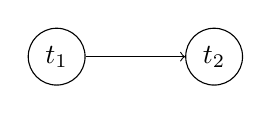
\begin{tikzpicture}[
      node distance=2cm
      ]
      \node[circle, draw] (t1) at (0,0) {\( t_1 \)};
      \node[circle, draw, right of=t1] (t2) {\( t_2 \)};

      \draw[->] (t1) to node[above] {} (t2);
    \end{tikzpicture}
  \end{figure}

  \smallskip
  Siccome il grafo è aciclico, allora \( \mathrm{S_1} \) è CSR e, quindi, \( \mathrm{S_1} \) è VSR.
}

\esempio{}{
  Consideriamo lo schedule:
  \[
    \mathrm{S_2 = r_1(x); \; w_1(x); \; w_3(x); \; r_2(y); \; r_3(y); \; w_3(y); \; w_1(y); \;
    r_2(x);}
  \] 

  Verifichiamo se \( \mathrm{S_2} \) è VSR e per farlo vediamo se prima è CSR controllando
  l'insieme dei conflitti:
  \[
    \begin{aligned}
      \texttt{CONFLITTI}(\mathrm{S_2}) =& 
      \{
        (\mathrm{r_1(x), w_3(x)}),\;
        (\mathrm{w_1(x), w_3(x)}),\;
        (\mathrm{w_1(x), r_2(x)}), \\
                             &(\mathrm{w_3(x), r_2(x)}),\;
                             (\mathrm{r_2(y), w_3(y)}),\;
                             (\mathrm{r_2(y), w_1(y)}), \\
                             &(\mathrm{r_3(y), w_1(y)}),\;
                             (\mathrm{w_3(y), w_1(y)})
                           \} 
    \end{aligned}
  \]

  Costruiamo il grafo dei conflitti:
  \begin{figure}[H]
    \centering
    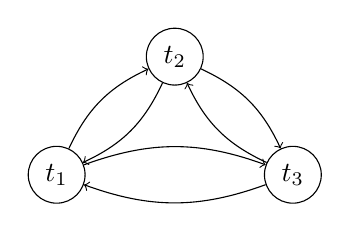
\begin{tikzpicture}
      \node[circle, draw] (t1) at (0,0) {\( t_1 \)};
      \node[circle, draw] (t2) at (1.5,1.5) {\( t_2 \)};
      \node[circle, draw] (t3) at (3,0) {\( t_3 \)};

      \draw[->] (t1) edge [bend left=20] node[above] {} (t2);
      \draw[->] (t2) edge [bend left=20] node[above] {} (t1);
      \draw[->] (t1) edge [bend left=20] node[above] {} (t3);
      \draw[->] (t3) edge [bend left=20] node[above] {} (t1);
      \draw[->] (t3) edge [bend left=20] node[above] {} (t2);
      \draw[->] (t2) edge [bend left=20] node[above] {} (t3);
    \end{tikzpicture}
  \end{figure}
  \noindent
  Il grafo è ciclico, quindi \( \mathrm{S_2} \) \textbf{non è conflict-serializzabile} e di
  conseguenza \( \mathrm{S_2} \) \textbf{non è view-serializzabile}.
}

\esempio{}{
    Consideriamo lo schedule:
  \[
    \begin{aligned}
      \mathrm{S_3} =& \mathrm{r_1(x)}; \; \mathrm{r_2(x)}; \; \mathrm{w_2(x)}; \; \mathrm{r_3(x)}; \; \mathrm{r_4(z)}; \; \mathrm{w_1(x)}; \; \mathrm{w_3(y)}; \;
      \mathrm{w_3(x)}; \; \mathrm{w_1(y)};\\
           &\mathrm{w_5(x)}; \; \mathrm{w_1(z)}; \; \mathrm{w_5(y)}; \; \mathrm{r_5(z)};
    \end{aligned}
  \] 
  Verifichiamo se \( \mathrm{S_3} \) è VSR, per farlo vediamo se prima è CSR controllando
  l'insieme dei conflitti:
  \[
    \begin{aligned}
      \texttt{CONFLITTI}(\mathrm{S_3}) =& \{
        (\mathrm{r_1(x), w_2(x)}),\;
        (\mathrm{r_1(x), w_3(x)}),\;
        (\mathrm{r_1(x), w_5(x)}), \\
                      &(\mathrm{r_2(x), w_1(x)}),\;
        (\mathrm{r_2(x), w_3(x)}),\;
        (\mathrm{r_2(x), w_5(x)}), \\
                      &(\mathrm{w_2(x), r_3(x)}),\;
        (\mathrm{w_2(x), w_1(x)}),\;
        (\mathrm{w_2(x), w_3(x)}), \\
                      &(\mathrm{w_2(x), w_5(x)}),\;
        (\mathrm{r_3(x), w_1(x)}),\;
        (\mathrm{r_3(x), w_5(x)}), \\
                      &(\mathrm{r_4(z), w_1(z)}),\;
        (\mathrm{w_1(x), w_3(x)}),\;
        (\mathrm{w_1(x), w_5(x)}), \\
                      &(\mathrm{w_3(y), w_1(y)}),\;
        (\mathrm{w_3(y), w_5(y)}),\;
        (\mathrm{w_3(x), w_5(x)}), \\
                      &(\mathrm{w_1(y), w_5(y)}),\;
        (\mathrm{w_1(z), r_5(z)})
      \} 
    \end{aligned}
  \] 
  Il grafo dei conflitti è ciclico, allora \( \mathrm{S_3} \) \textbf{non è conflict-serializzabile} e di conseguenza \( \mathrm{S_3} \) \textbf{non è view-serializzabile}.
}

\subsection{Locking a due fasi stretto}
Il \textbf{locking a due fasi} (2PL) è il metodo applicato nei sistemi reali per la gestione dell'esecuzione concorrente delle transazioni perchè non richiede di conoscere in anticipo l'esito delle transazioni.\\[0.2ex]
\hl{Il locking a due fasi è un sottoinsieme della conflict-serializzabilità}.

\smallskip
Gli aspetti che caratterizzano il locking a due fasi sono i seguenti:
\begin{itemize}[label=$\triangleright$, itemsep=\medskipamount]
  \item \textbf{meccanismo di base per la gestione dei lock}: si basa sull'introduzione di alcune primitive di lock che consentono alle transazioni di bloccare le risorse sulle quali vogliono agire con operazioni di lettura e scrittura. 
  
  Le primitive di lock sono le seguenti:
  \begin{itemize}[label=$\diamond$, itemsep=\smallskipamount]
    \item \( \mathbf{r\_lock_K(x)} \): richiesta di un lock \textbf{condiviso} da parte della
      transazione \( \mathrm{t_K} \) sulla risorsa \( \mathrm{x} \) per eseguire una lettura

    \item \( \mathbf{w\_lock_K(x)} \): richiesta di un lock \textbf{esclusivo} da parte della
      transazione \( \mathrm{t_K} \) sulla risorsa \( \mathrm{x} \) per eseguire una scrittura

    \item \(\mathbf{ unlock_K(x)} \): richiesta da parte della transazione \( \mathrm{t_K} \) di liberare la risorsa \( \mathrm{x} \) da un precedente lock
  \end{itemize}
  
  \smallskip
  Le transazioni devono seguire le seguenti regole per applicare le primitive di
  lock:
  \begin{itemize}[label=$\circ$, itemsep=\smallskipamount]
    \item ogni \textbf{lettura} deve essere preceduta da un \( \mathrm{r\_lock} \) e seguita
      da un \( \mathrm{unlock} \). 
      
      Sono ammessi più \( \mathrm{r\_lock} \) contemporanei sulla stessa risorsa (lock condiviso)

    \item ogni \textbf{scrittura} deve essere preceduta da un \( \mathrm{w\_lock} \) e seguita da un \( \mathrm{unlock} \). 
    
    Non sono ammessi più \( \mathrm{w\_lock} \) (oppure \( \mathrm{w\_lock} \) e \( \mathrm{r\_lock} \)) contemporanei sulla stessa risorsa (lock esclusivo)
  \end{itemize}
  
  Se una transazione segue le precedenti regole, allora si dice \textbf{ben formata} rispetto al locking.

  \item \textbf{politica di concessione dei lock sulle risorse}: il gestore dei lock (o gestore della concorrenza) mantiene per ogni risorsa \( \mathrm{x} \) le seguenti informazioni:
  \begin{itemize}[label=$\diamond$, itemsep=\smallskipamount]
    \item \textbf{stato}: \( \mathrm{s(x)} \in \left\{ \mathrm{libero}, \mathrm{r\_lock}, \mathrm{w\_lock} \right\} \) 

    \item \textbf{transazioni in r\_lock}: \( \mathrm{c(x)} = \left( \mathrm{t_1, \dots, t_n} \right)  \), dove \( \mathrm{t_1, \ldots, t_n} \) hanno un \( \mathrm{r\_lock} \) su \( \mathrm{x} \)
  \end{itemize}
  Il comportamento del gestore dei lock è descritto dalla seguente tablella:
  \begin{figure}[H]
    \centering
    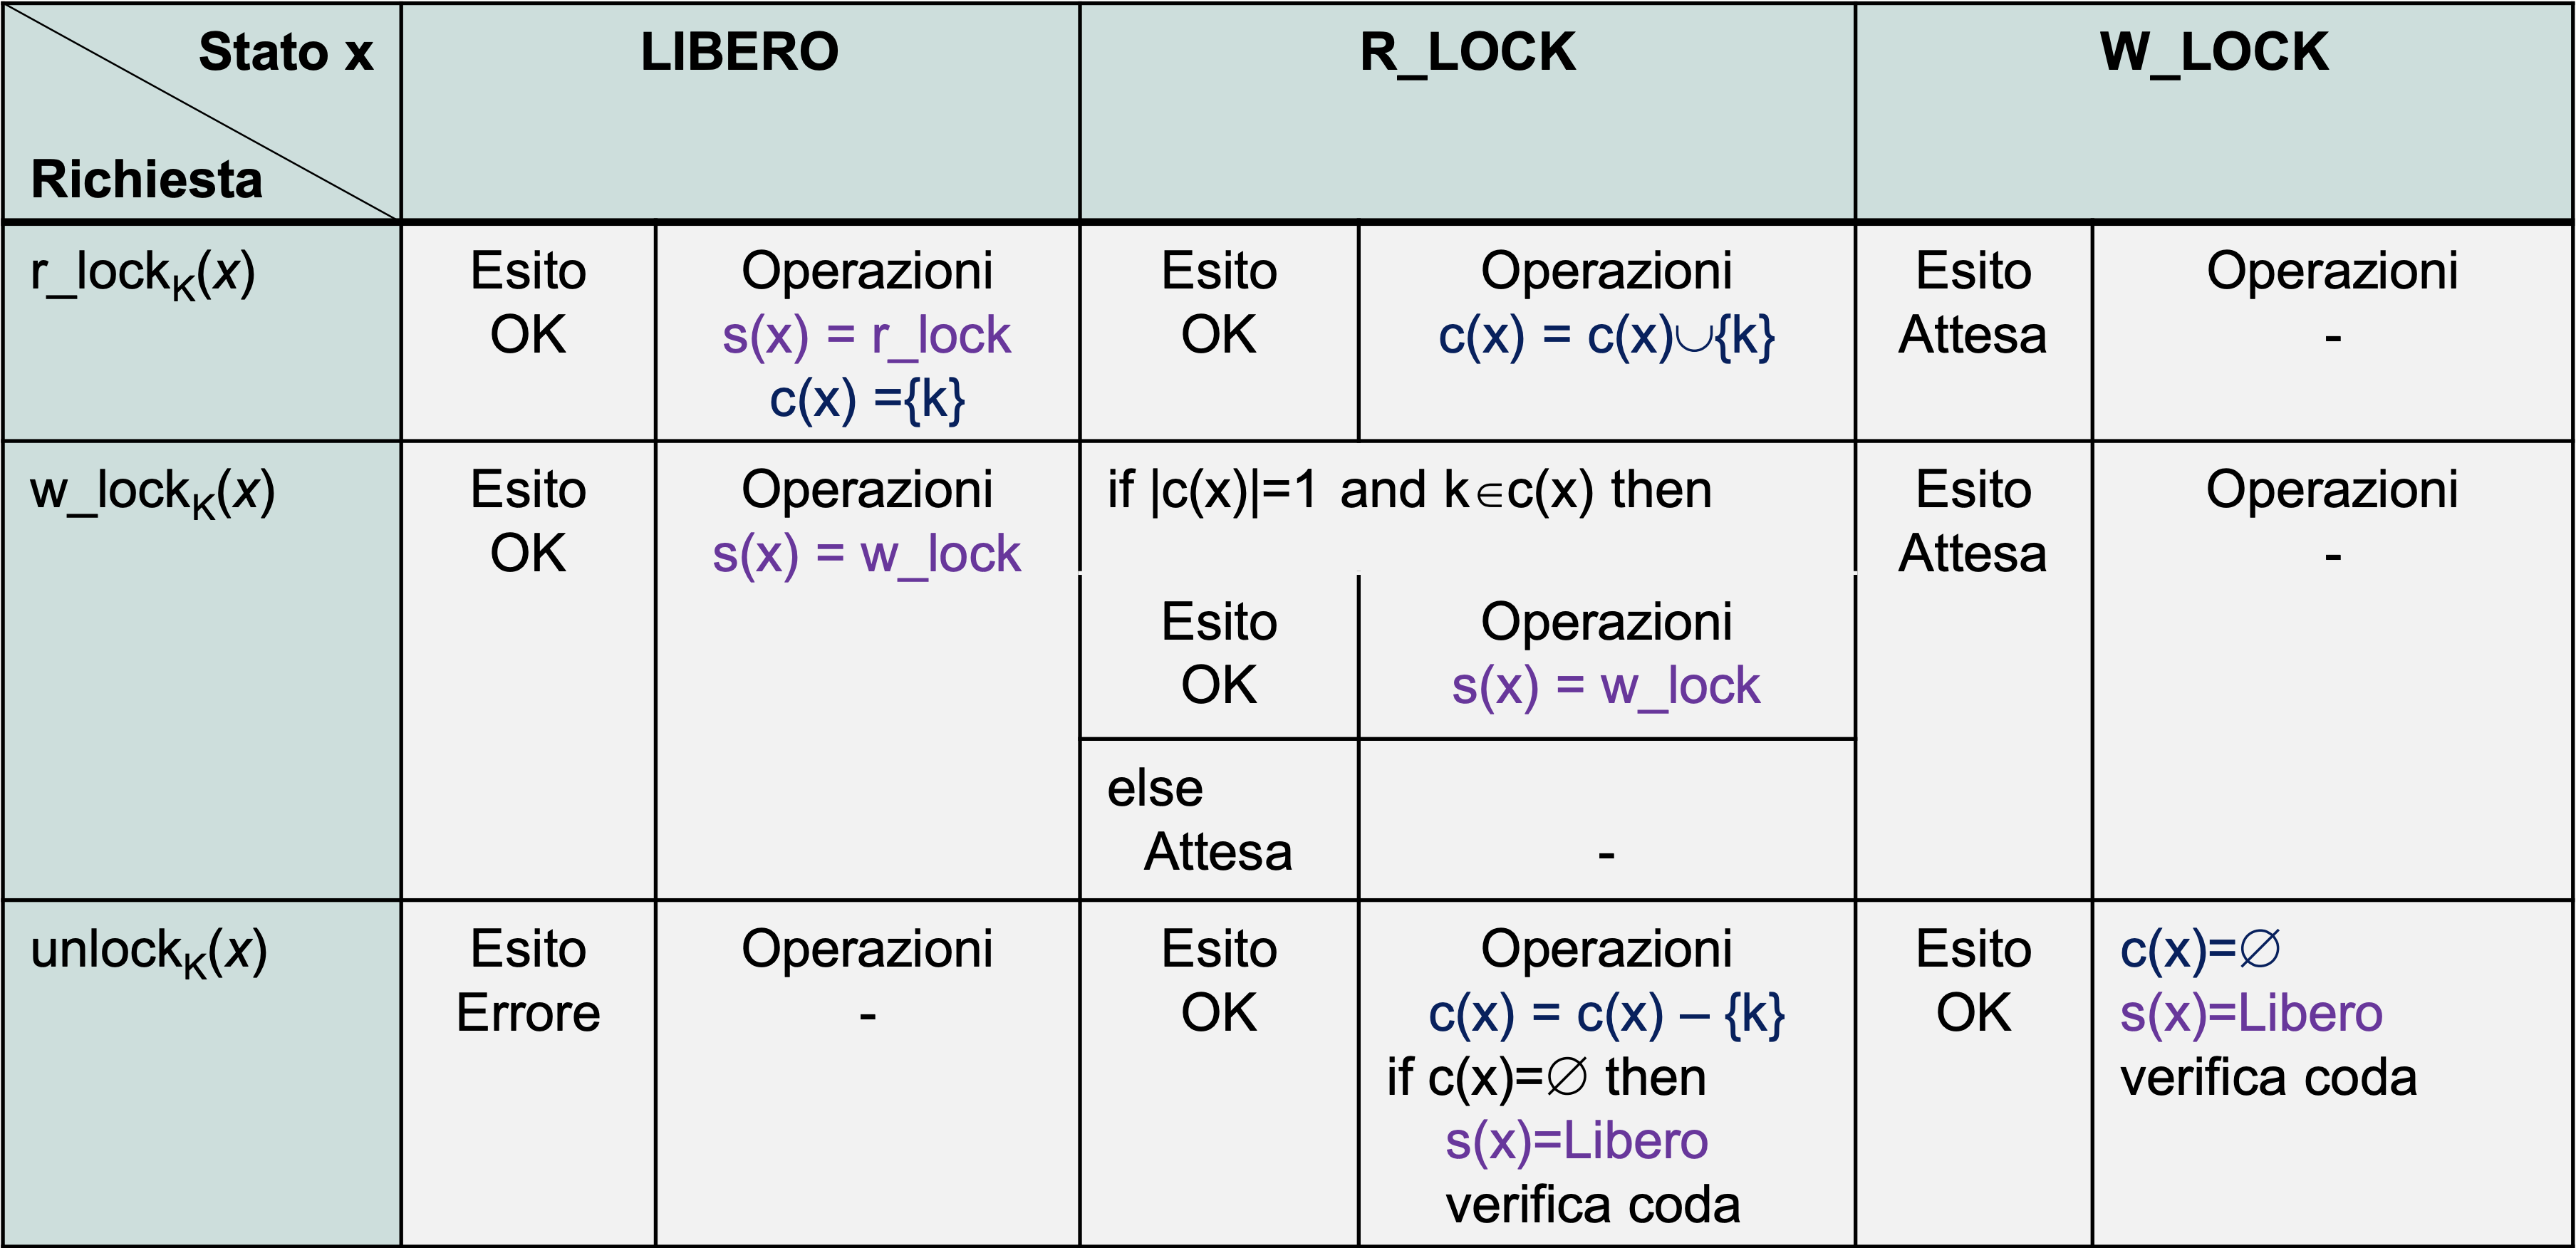
\includegraphics[width=0.5\textwidth]{images/gestore-lock.png}
  \end{figure}

  \item \textbf{regola che garantisce la serializzabilità}: una transazione dopo aver rilasciato un lock non può acquisirne altri.
  
  Questa regola è visualizzata dal seguente grafico:
  \begin{figure}[H]
    \centering
    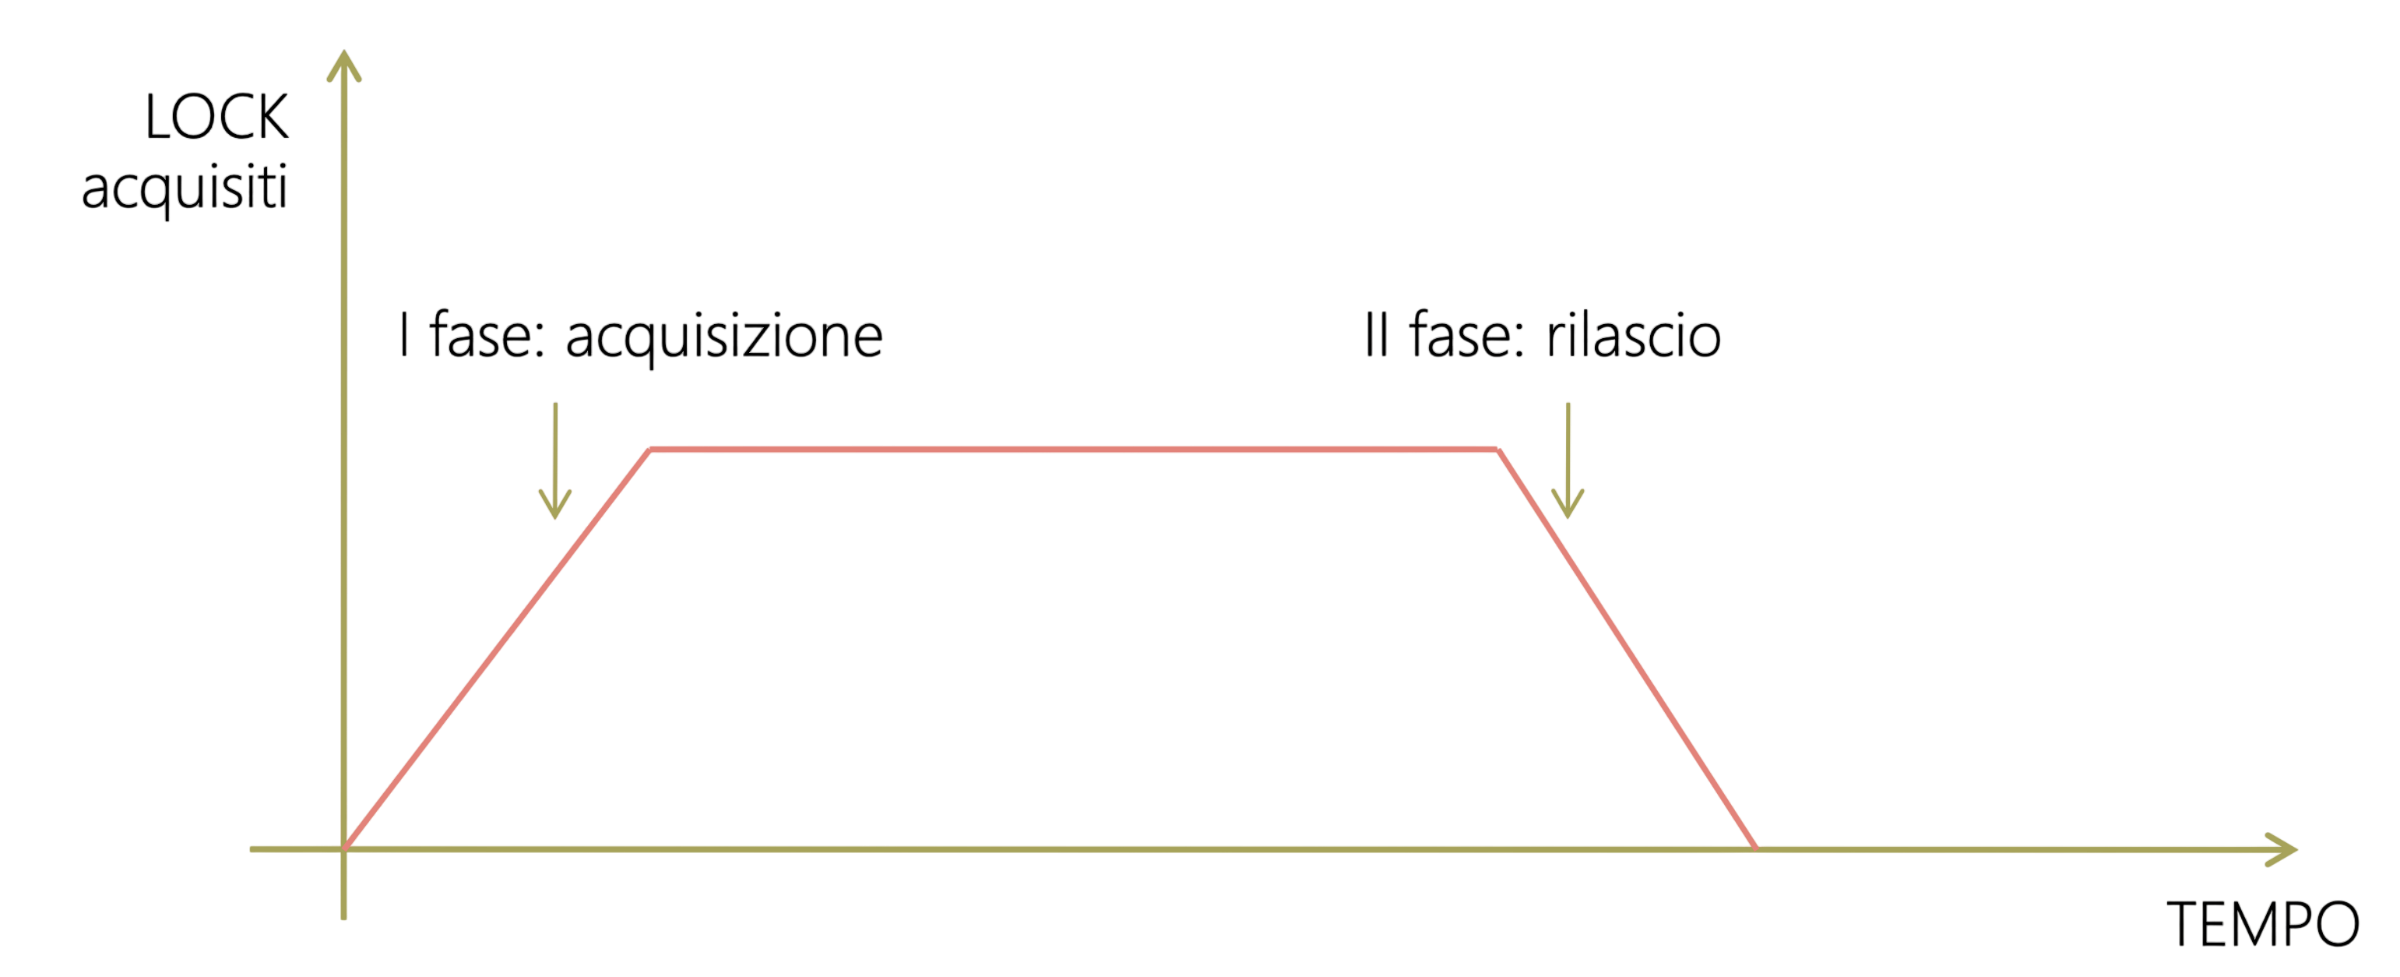
\includegraphics[width=0.6\textwidth]{images/locking-due-fasi.png}
    \caption{locking a due fasi}
  \end{figure}
\end{itemize}

\esempio{perdita di aggiornamento}{
    Consideriamo le seguenti transazioni:
  \[
  \begin{aligned}
    \mathrm{t_1}:\; & \mathrm{r_1(x)}; \; \mathrm{w_1(x)} \\
    \mathrm{t_2}:\; & \mathrm{r_2(x)}; \; \mathrm{w_2(x)}
  \end{aligned}
  \]

  Eseguire lo schedule:
  \[
    \mathbf{S_{pa}:\; r_1(x); \; r_2(x); \; w_2(x); \; w_1(x);}
  \]

  \begin{enumerate}[itemsep=\smallskipamount]
    \item \( \mathrm{r_1(x)} \) richiede un \( \mathrm{r\_lock_1(x)} \) 
    \item \( \mathrm{r_2(x)} \) richiede un \( \mathrm{r\_lock_2(x)} \)
    \item \( \mathrm{w_2(x)} \) richiede un \( \mathrm{w\_lock_2(x)} \), ma lo stato \( \mathrm{s(x) = r\_lock} \), con \( \mathrm{c(x)} = \left\{ \mathrm{t_1, t_2} \right\} \), quindi, \( \mathrm{w_2(x)} \) per ottenere \( \mathrm{w\_lock_2(x)} \) deve attendere che \( \mathrm{t_1} \) rilasci \( \mathrm{r\_lock(x)} \) ma se \( \mathrm{t_1} \) rilascia \( \mathrm{r\_lock(x)} \) e, quindi, inizierebbe la sua fase discendente impedendogli di acquisire altri lock e di conseguenza \( \mathrm{w\_lock_1(x)} \) non è più possibile per la serializzabilità del 2PL
  \end{enumerate}

  \smallskip
  Di conseguenza questo schedule \textbf{non è 2PL}.
}

Il locking a due fasi stretto (strict 2PL) è una variante del locking a due fasi che introduce una condizione aggiuntiva per rimuovere la necessità dell'ipotesi di commit-proiezione. 

La condizione aggiuntiva è la seguente: Una transazione può rilasciare i lock solo quando ha eseguito correttamente un \texttt{commit} o un \texttt{rollback}.

\begin{figure}[H]
  \centering
  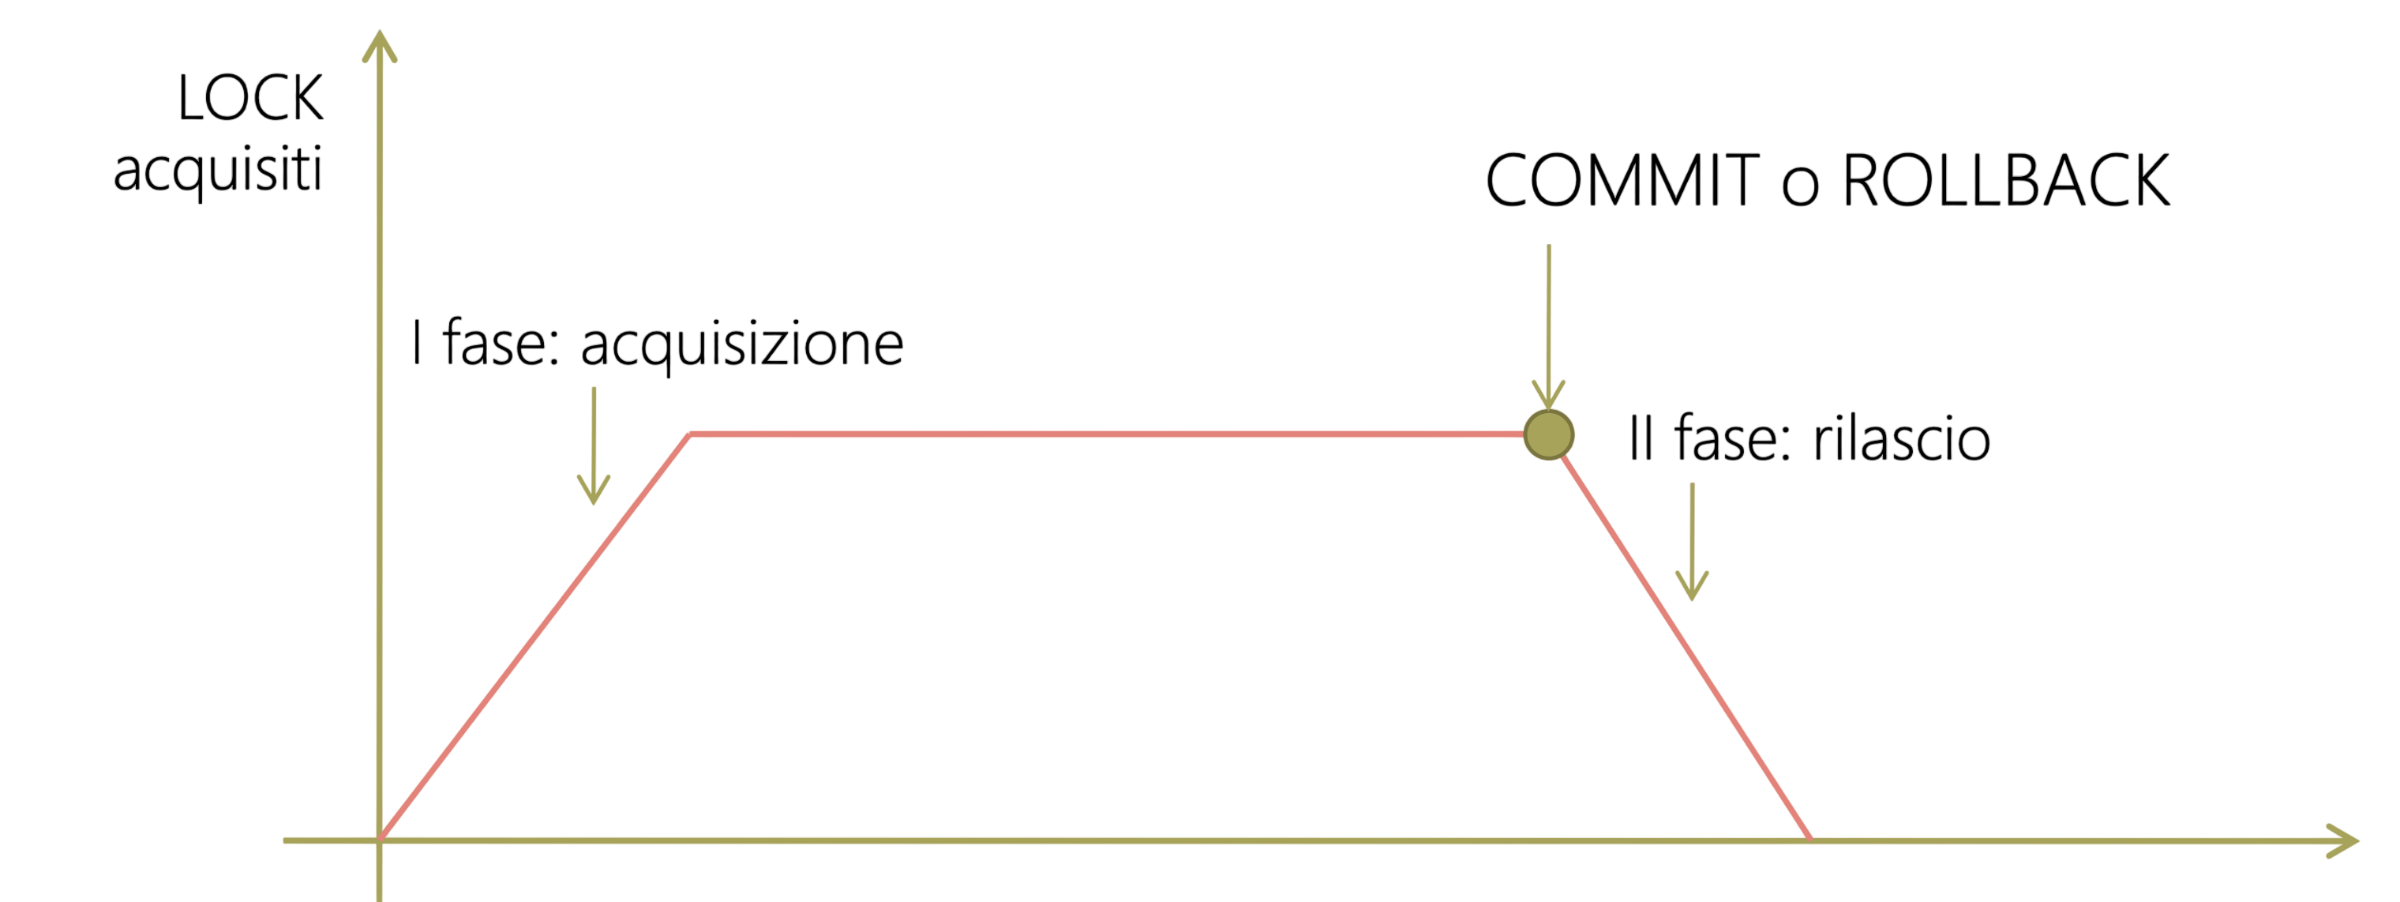
\includegraphics[width=0.6\textwidth]{images/locking-due-fasi-stretto.png}
  \caption{locking a due fasi stretto}
\end{figure}

\subsection{Blocco critico (deadlock)}
Il \textbf{blocco critico} è una situazione di blocco che si verifica nell'esecuzione di transazioni concorrenti quando:
\begin{itemize}[label=$\circ$, itemsep=\smallskipamount]
  \item due transazioni hanno bloccato delle risorse:
    \begin{itemize}
      \item \( \mathrm{t_1} \) ha bloccato \( \mathrm{r_1} \)

      \item \( \mathrm{t_2} \) ha bloccato \( \mathrm{r_2} \)
    \end{itemize}

  \item \( \mathrm{t_1} \) è in attesa sulla risorsa \( \mathrm{r_2} \) e \( \mathrm{t_2} \) è in attesa sulla risorsa \( \mathrm{r_1} \)
\end{itemize}

Se il numero medio di tuple per tabella è \( \mathrm{n} \) e la granularità del lock (numero di risorse che possono essere bloccate) è la tupla, la probabilità che si verifichi un lock tra due transazioni è:
\[
  \mathbf{P(\text{deadlock di lunghezza 2}) = \frac{1}{n^2}}
\]

\esempio{deadlock}{
  Un esempio di deadlock utilizzando il locking a due fasi stretto è il seguente:
  \begin{figure}[H]
    \centering
    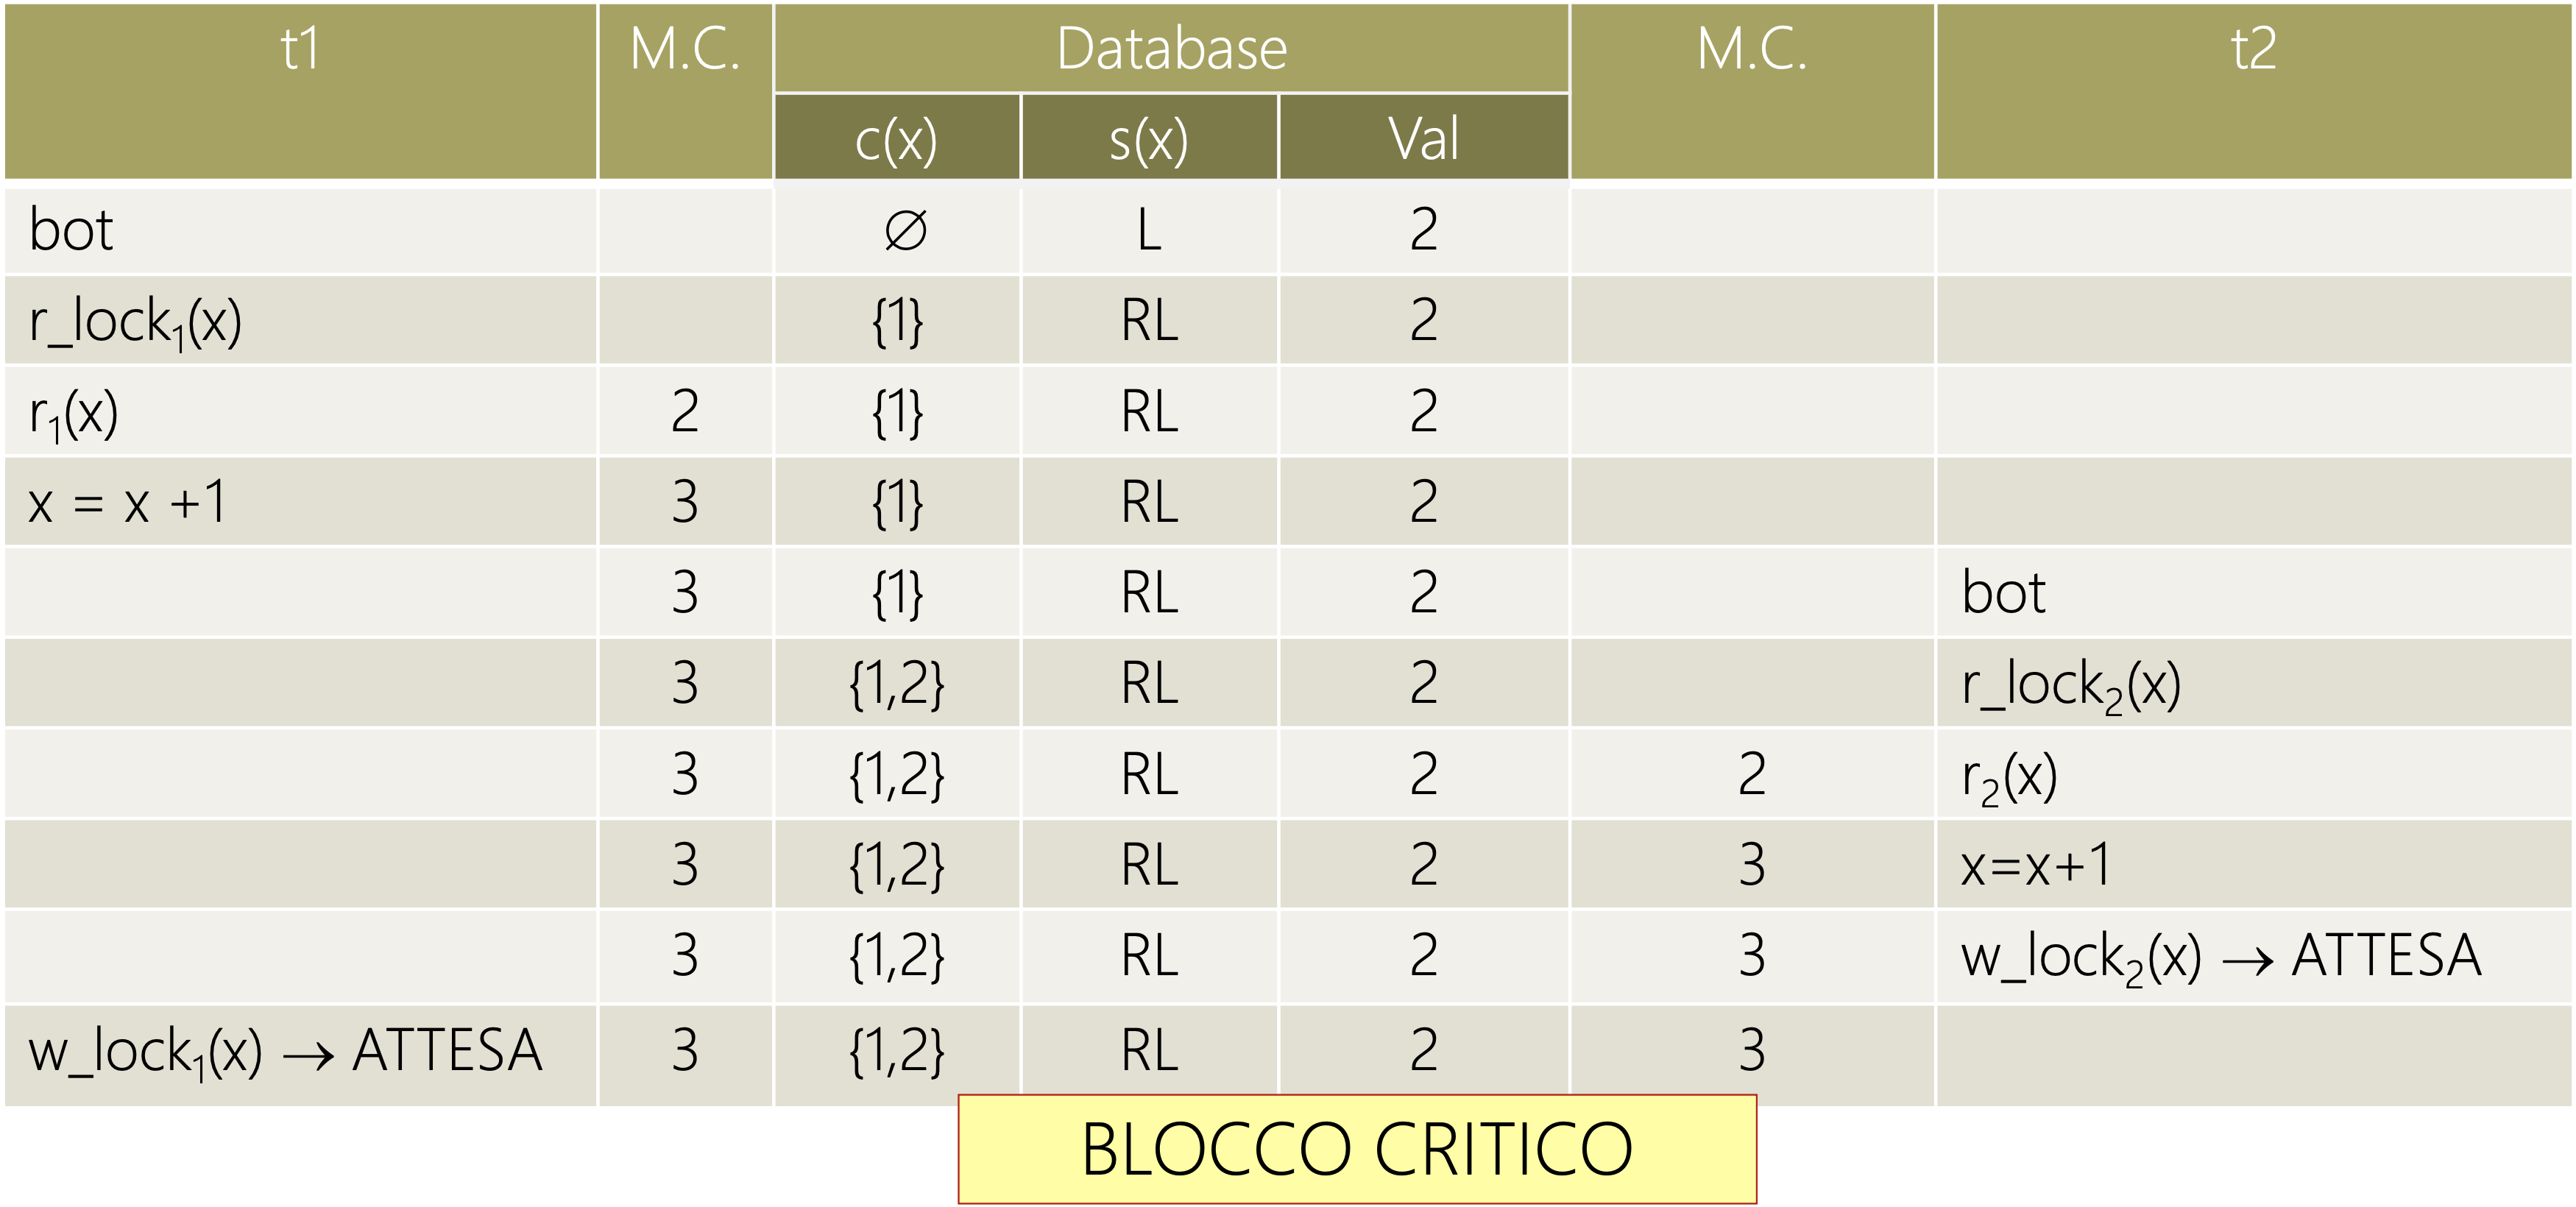
\includegraphics[width=0.7\textwidth]{images/deadlock-locking-due-fasi-stretto.png}
  \end{figure}
}

\noindent
Le tecniche per risolvere i deadlock sono le seguenti:
\begin{itemize}[label=$\diamond$, itemsep=\smallskipamount]
  \item \textbf{timeout}: se una transazione è in attesa su una risorsa da troppo tempo 
    viene abortita

  \item \textbf{prevenzione}: 
  \begin{itemize}[itemsep=\smallskipamount]
    \item una transazione blocca tutte le risorse a cui deve accedere in lettura o
      scrittura in una sola volta (o blocca tutto o non blocca nulla)

    \item ogni transazione \( \mathrm{t_i} \) acquisisce un timestamp \( \mathrm{TS_i} \) all'inizio della sua esecuzione. 
    
    La transazione \( \mathrm{t_i} \) può attendere una risorsa bloccata da \( \mathrm{t_j} \) solo se vale una certa condizione sui timestamp (es. \( \mathrm{TS_i < TS_j} \)), altrimenti \( \mathrm{t_i} \) viene abortita e fatta ripartire con lo stesso timestamp
  \end{itemize}

  \item \textbf{rilevamento}: si esegue un'analisi periodica della tabella di lock per rilevare la presenza di un deadlock che corrisponde ad un ciclo nel grafo delle relazioni di attesa.
  
  Questa tecnica è la più utilizzata nei sistemi reali.
\end{itemize}

Inoltre la scelta di gestire i lock in lettura come lock condivisi introduce il problema della \textbf{starvation} che tuttavia nel contesto delle DMBS risulta poco probabile, ma comunque risolvibile con le tecniche precedenti.

\definizione{starvation}{
  Se una risorsa \( \mathrm{x} \) viene costantemente bloccata da una sequenza di transazioni che acquisiscono \( \mathrm{r\_lock} \) su \( \mathrm{x} \), un'eventuale transazione in attesa di scrivere su \( \mathrm{x} \) viene bloccata per un lungo periodo fino alla fine della sequenza di letture.
  \begin{figure}[H]
    \centering
    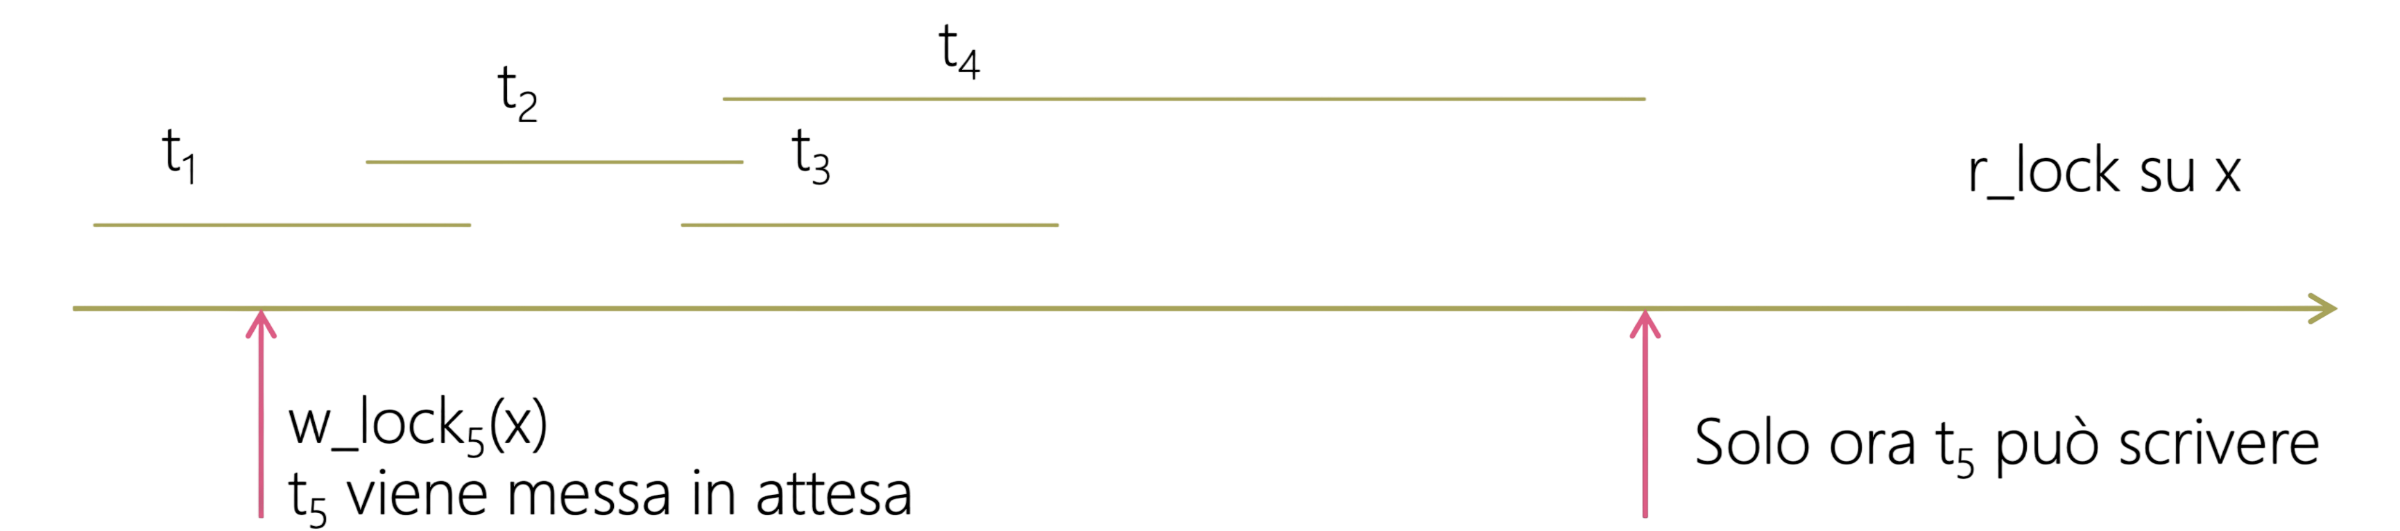
\includegraphics[width=0.7\textwidth]{images/starvation.png}
  \end{figure}
}

\subsection{Gestione della concorrenza in SQL}
Siccome risulta molto pesante per il sistema gestire l'esecuzione concorrente di
transazioni con una conseguente diminuzione delle prestazioni, SQL prevede la 
possibilità di \textbf{rinunciare del tutto o in parte al controllo di concorrenza}
per aumentare le prestazioni del sistema.\\[0.2ex]
È quindi possibile, a livello di una singola transazione, decidere di \textbf{tollerare alcune anomalie} di esecuzione concorrente.

\smallskip
La seguente tabella mostra le possibili combinazioni di anomalie che si possono tollerare:
\begin{figure}[H]
  \centering
  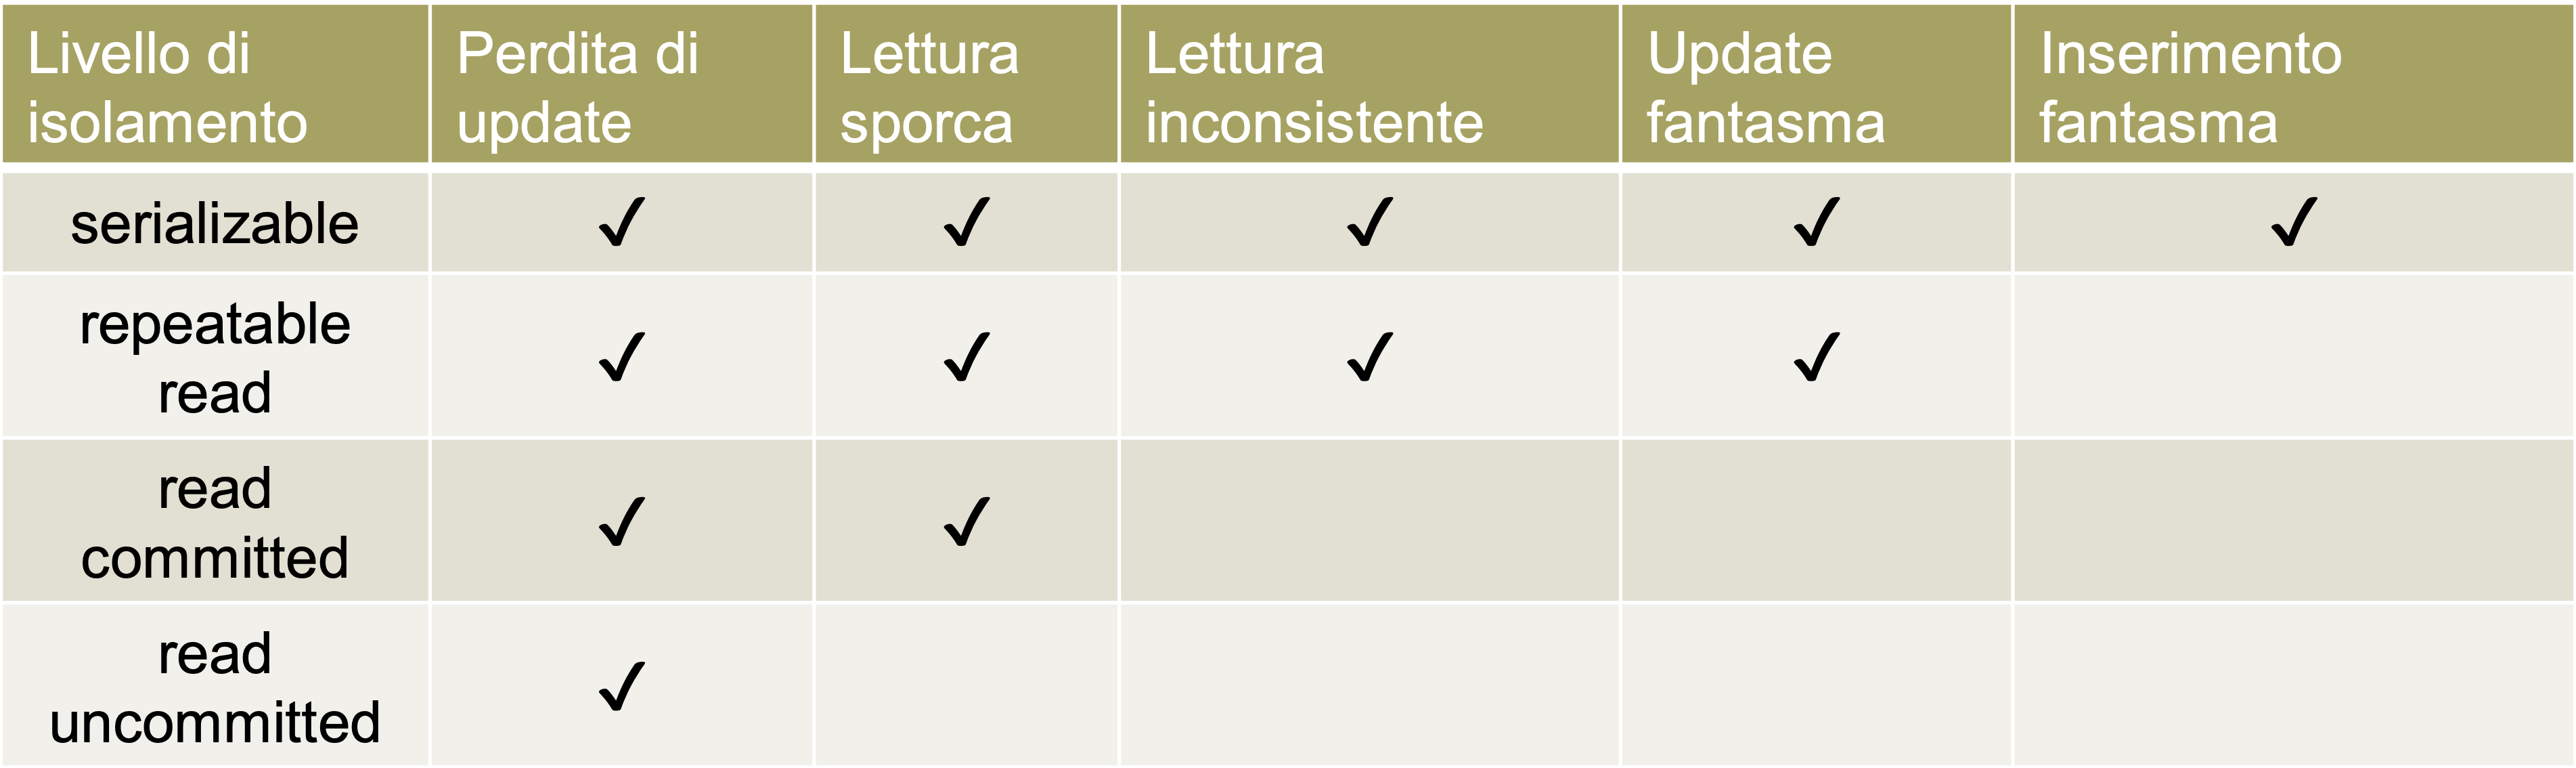
\includegraphics[width=0.7\textwidth]{images/anomalie-tollerate-SQL.png}
  \caption{Anomalie tollerate in SQL}
\end{figure}

\vario{Nota}{
    \begin{itemize}[label=$\triangleright$, itemsep=\smallskipamount]
        \item tutti i livelli richiedono il 2PL stretto per le scritture
        \item \textbf{serializable}: richiede il 2PL stretto anche per le letture e applica il lock sulle tabelle per evitare l'inserimento fantasma
        \item \textbf{repeatable read}: applica il 2PL stretto anche per le letture, ma applica i lock a livello di tupla e non di tabella.
        
        Consente inserimenti e, quindi, non evita l'anomalia di inserimento fantasma.

        \textcolor{red}{\textbf{Attenzione}}: in PostgreSQL la repeatable read è implementata in modo più stringente che evita anche l'anomalia di inserimento fantasma
        \item \textbf{read committed}: richiede lock condivisi per le letture, ma non il 2PL stretto
        \item \textbf{read uncommitted}: non applica lock in lettura
    \end{itemize}
}